% IEEE two-column journal version of the paper (IEEEtran, journal mode).
% Numbers come only from ../autogen_numbers.tex (generated from results/full/);
% figures come only from ../../figures/ (generated by experiments/make_figures.py);
% references from refs_ieee.bib, generated from ../references.bib by experiments/build_paper.py.
\documentclass[journal]{IEEEtran}
\usepackage[utf8]{inputenc}
\usepackage[T1]{fontenc}
\usepackage{cite}
\usepackage{amsmath,amssymb}
\usepackage{graphicx}
\usepackage{booktabs}
\usepackage{array}
\usepackage{xcolor}
\usepackage[hidelinks]{hyperref}

\graphicspath{{../../figures/}}
% Auto-generated by experiments/make_numbers.py from results/full/.
% Do not edit by hand.

\newcommand{\Nreps}{30}  % IBM replicates per condition
\newcommand{\MSmall}{50}  % players, small setting
\newcommand{\NSmall}{10}  % umpires, small setting
\newcommand{\WinSmall}{100000}  % window, small IBM (generations)
\newcommand{\BurnSmall}{5000}  % burn-in, small IBM
\newcommand{\WinLarge}{5000}  % window, large IBM
\newcommand{\BurnLarge}{1000}  % burn-in, large IBM
\newcommand{\TBurnMF}{10000}  % mean-field burn-in
\newcommand{\TWinMF}{10000}  % mean-field window
\newcommand{\MuMF}{0.01}  % mean-field exploration rate
\newcommand{\BoneOD}{0.25}  % B1 target OD
\newcommand{\BonePC}{0.75}  % B1 target PC
\newcommand{\BoneDev}{4.8\times 10^{-12}}  % B1 max deviation
\newcommand{\BtwoDev}{2.4\times 10^{-11}}  % B2 max deviation
\newcommand{\BoneStarts}{20}  % random starts
\newcommand{\PrintedOC}{1.000}  % OC under printed weighting at y=0
\newcommand{\HopfMuA}{0.0616}  % Hopf in mu=nu, A=2
\newcommand{\HopfMuB}{0.0314}  % Hopf in mu=nu, A=0.7
\newcommand{\HopfPerA}{62.8}  % period at Hopf, A=2
\newcommand{\PerSlow}{9437}  % period mu=1e-4, A=2
\newcommand{\SlowOCmax}{1.000}  % max OC mu=1e-4
\newcommand{\SlowPDmax}{0.858}  % max PD mu=1e-4
\newcommand{\PerViolet}{136.5}  % period mu=0.02
\newcommand{\VioletOC}{0.923}  % max OC, mu=0.02
\newcommand{\VioletPC}{0.697}  % max PC, mu=0.02
\newcommand{\VioletOD}{0.268}  % max OD, mu=0.02
\newcommand{\VioletPD}{0.438}  % max PD, mu=0.02
\newcommand{\VioletYmin}{0.047}  % min honest, mu=0.02
\newcommand{\SlowDistNine}{0.142}  % min distance to state 9, A=2
\newcommand{\SlowDistEight}{0.843}  % min distance to state 8, A=2
\newcommand{\SlowBDistEight}{0.022}  % min distance to state 8, A=0.7
\newcommand{\SlowBDistNine}{0.998}  % min distance to state 9, A=0.7
\newcommand{\PerSlowB}{4508}  % period mu=1e-4, A=0.7
\newcommand{\yODA}{0.167}  % y_OD at A=2
\newcommand{\yPD}{0.333}  % y_PD
\newcommand{\yODB}{0.600}  % y_OD at A=0.7
\newcommand{\MarkovRatio}{2.541}  % Markov H:C at N=10
\newcommand{\MarkovRatioFinM}{2.540}  % Markov with 1/M neutral player fixation
\newcommand{\MarkovNdiff}{4}  % number of differing entries
\newcommand{\BthreeRatio}{2.030}  % IBM H:C at mu=1e-3
\newcommand{\BthreeRatioLo}{2.003}  % IBM H:C at mu=1e-3 (95% CI low)
\newcommand{\BthreeRatioHi}{2.057}  % IBM H:C at mu=1e-3 (95% CI high)
\newcommand{\BthreeRatioB}{2.318}  % IBM H:C at mu=3e-4
\newcommand{\BthreeRatioBLo}{2.280}  % IBM H:C at mu=3e-4 (95% CI low)
\newcommand{\BthreeRatioBHi}{2.358}  % IBM H:C at mu=3e-4 (95% CI high)
\newcommand{\BthreeRatioC}{2.459}  % IBM H:C at mu=1e-4
\newcommand{\BthreeRatioCLo}{2.418}  % IBM H:C at mu=1e-4 (95% CI low)
\newcommand{\BthreeRatioCHi}{2.499}  % IBM H:C at mu=1e-4 (95% CI high)
\newcommand{\BthreeDouble}{2.032}  % H:C with doubled window
\newcommand{\BthreeDoubleLo}{2.014}  % H:C with doubled window (95% CI low)
\newcommand{\BthreeDoubleHi}{2.049}  % H:C with doubled window (95% CI high)
\newcommand{\EpisodesSteps}{6.0}  % episodes per 1e5 steps
\newcommand{\EpisodesStepsLo}{6.0}  % episodes per 1e5 steps (95% CI low)
\newcommand{\EpisodesStepsHi}{6.1}  % episodes per 1e5 steps (95% CI high)
\newcommand{\BthreeGens}{200000}  % generations per replicate
\newcommand{\PaperRatio}{2.15}  % paper simulated ratio
\newcommand{\BthreeSE}{0.0010}  % SE of ybar at 30 reps (B3)
\newcommand{\BfourOC}{0.534}  % large IBM late mean OC
\newcommand{\BfourOCLo}{0.510}  % large IBM late mean OC (95% CI low)
\newcommand{\BfourOCHi}{0.560}  % large IBM late mean OC (95% CI high)
\newcommand{\BfourPC}{0.186}  % large IBM late mean PC
\newcommand{\BfourPCLo}{0.170}  % large IBM late mean PC (95% CI low)
\newcommand{\BfourPCHi}{0.201}  % large IBM late mean PC (95% CI high)
\newcommand{\BfourOD}{0.050}  % large IBM late mean OD
\newcommand{\BfourODLo}{0.049}  % large IBM late mean OD (95% CI low)
\newcommand{\BfourODHi}{0.052}  % large IBM late mean OD (95% CI high)
\newcommand{\BfourPD}{0.229}  % large IBM late mean PD
\newcommand{\BfourPDLo}{0.216}  % large IBM late mean PD (95% CI low)
\newcommand{\BfourPDHi}{0.242}  % large IBM late mean PD (95% CI high)
\newcommand{\BfourCorrupt}{0.541}  % large IBM late mean corrupt
\newcommand{\BfourCorruptLo}{0.535}  % large IBM late mean corrupt (95% CI low)
\newcommand{\BfourCorruptHi}{0.545}  % large IBM late mean corrupt (95% CI high)
\newcommand{\FermiCorrupt}{0.544}  % Fermi mean-field corrupt fraction
\newcommand{\FermiRe}{-0.0081}  % leading eigenvalue real part
\newcommand{\FermiIm}{0.0089}  % leading eigenvalue imaginary part
\newcommand{\FermiPer}{705}  % damped oscillation period (gen)
\newcommand{\FermiDecay}{124}  % decay time (gen)
\newcommand{\LargeReps}{10}  % large IBM replicates (B4)
\newcommand{\ValMA}{500}  % validation M
\newcommand{\ValRmsA}{0.113}  % validation RMS
\newcommand{\ValMB}{2000}  % validation M
\newcommand{\ValRmsB}{0.047}  % validation RMS
\newcommand{\ValMC}{8000}  % validation M
\newcommand{\ValRmsC}{0.025}  % validation RMS
\newcommand{\ValMD}{32000}  % validation M
\newcommand{\ValRmsD}{0.011}  % validation RMS
\newcommand{\RhoC}{0.0133}  % critical rotation rate (fold, SNIC)
\newcommand{\RhoCApprox}{0.0137}  % small-mu formula
\newcommand{\RhoCErr}{2.5}  % relative error of formula (percent)
\newcommand{\RhoCy}{0.583}  % honesty at the fold (formula)
\newcommand{\RhoFtwo}{0.126}  % second fold
\newcommand{\FoldY}{0.582}  % honest fraction at the fold
\newcommand{\FoldOC}{0.957}  % OC at the fold
\newcommand{\FoldPC}{0.015}  % PC at the fold
\newcommand{\SnicSlope}{-0.478}  % log-log slope of period
\newcommand{\NHopfDefault}{0}  % Hopf points at default
\newcommand{\YbarZero}{0.581}  % mean honesty rho=0
\newcommand{\PCZero}{0.174}  % mean PC rho=0
\newcommand{\PerZero}{203.5}  % period rho=0
\newcommand{\YminZero}{0.020}  % min y on cycle rho=0
\newcommand{\RhoLastCycle}{0.0132}  % largest rho with a cycle
\newcommand{\YbarLastCycle}{0.586}  % mean honesty just below rho_c
\newcommand{\PCLastCycle}{0.036}  % mean PC just below rho_c
\newcommand{\DepthCZero}{0.245}  % min cooperation in episode, rho=0
\newcommand{\DepthCLast}{0.263}  % min cooperation in episode, near rho_c
\newcommand{\DepthYZero}{0.980}  % peak corruption rho=0
\newcommand{\DepthYLast}{0.955}  % peak corruption near rho_c
\newcommand{\RhoFirstEq}{0.0135}  % first rho with equilibrium
\newcommand{\YbarFirstEq}{0.606}  % honesty just above rho_c
\newcommand{\PCFirstEq}{0.016}  % PC just above rho_c
\newcommand{\YbarRhoFive}{0.868}  % honesty at rho=0.05
\newcommand{\PCRhoFive}{0.024}  % PC at rho=0.05
\newcommand{\YbarRhoTen}{0.921}  % honesty at rho=0.1
\newcommand{\PCRhoTen}{0.027}  % PC at rho=0.1
\newcommand{\YbarRhoTwenty}{0.957}  % honesty at rho=0.2
\newcommand{\PCRhoTwenty}{0.029}  % PC at rho=0.2
\newcommand{\RhoCOverMuA}{1.36}  % rho_c/mu at small mu, A=2.0
\newcommand{\MuMaxFoldA}{0.056}  % largest mu with two folds, A=2.0
\newcommand{\NHopfTwoparA}{2}  % Hopf points in two-parameter scan, A=2.0
\newcommand{\ApproxErrMaxA}{2.5}  % max rel err of formula for mu<=0.011, A=2.0
\newcommand{\RhoCOverMuB}{3.35}  % rho_c/mu at small mu, A=0.7
\newcommand{\MuMaxFoldB}{0.042}  % largest mu with two folds, A=0.7
\newcommand{\NHopfTwoparB}{2}  % Hopf points in two-parameter scan, A=0.7
\newcommand{\ApproxErrMaxB}{0.1}  % max rel err of formula for mu<=0.011, A=0.7
\newcommand{\RhoCLowH}{0.0160}  % rho_c at h=0.02
\newcommand{\RhoCHighH}{0.0017}  % rho_c at h=0.28
\newcommand{\RhoCMaxH}{0.04}  % h where rho_c is largest
\newcommand{\RhoCMax}{0.0165}  % largest rho_c
\newcommand{\YbarZeroLowH}{0.769}  % honesty rho=0 h=0.02
\newcommand{\YbarZeroHighH}{0.377}  % honesty rho=0 h=0.28
\newcommand{\GainLowH}{0.134}  % gain at rho=0.05, h=0.02
\newcommand{\GainHighH}{0.478}  % gain at rho=0.05, h=0.28
\newcommand{\HoneYSZero}{0.669}  % H1 ibm_small ybar rho=0
\newcommand{\HoneYSZeroLo}{0.665}  % H1 ibm_small ybar rho=0 (95% CI low)
\newcommand{\HoneYSZeroHi}{0.673}  % H1 ibm_small ybar rho=0 (95% CI high)
\newcommand{\HoneYSMax}{0.978}  % H1 ibm_small ybar rho max
\newcommand{\HoneYSMaxLo}{0.978}  % H1 ibm_small ybar rho max (95% CI low)
\newcommand{\HoneYSMaxHi}{0.979}  % H1 ibm_small ybar rho max (95% CI high)
\newcommand{\HoneEpSZero}{3.63}  % H1 ibm_small episodes rho=0
\newcommand{\HoneEpSZeroLo}{3.59}  % H1 ibm_small episodes rho=0 (95% CI low)
\newcommand{\HoneEpSZeroHi}{3.67}  % H1 ibm_small episodes rho=0 (95% CI high)
\newcommand{\HoneEpSMax}{0.29}  % H1 ibm_small episodes max
\newcommand{\HoneEpSMaxLo}{0.27}  % H1 ibm_small episodes max (95% CI low)
\newcommand{\HoneEpSMaxHi}{0.31}  % H1 ibm_small episodes max (95% CI high)
\newcommand{\HoneYLZero}{0.458}  % H1 ibm_large ybar rho=0
\newcommand{\HoneYLZeroLo}{0.457}  % H1 ibm_large ybar rho=0 (95% CI low)
\newcommand{\HoneYLZeroHi}{0.460}  % H1 ibm_large ybar rho=0 (95% CI high)
\newcommand{\HoneYLMax}{0.876}  % H1 ibm_large ybar rho max
\newcommand{\HoneYLMaxLo}{0.876}  % H1 ibm_large ybar rho max (95% CI low)
\newcommand{\HoneYLMaxHi}{0.876}  % H1 ibm_large ybar rho max (95% CI high)
\newcommand{\HoneEpLZero}{10.07}  % H1 ibm_large episodes rho=0
\newcommand{\HoneEpLZeroLo}{9.60}  % H1 ibm_large episodes rho=0 (95% CI low)
\newcommand{\HoneEpLZeroHi}{10.54}  % H1 ibm_large episodes rho=0 (95% CI high)
\newcommand{\HoneEpLMax}{0.00}  % H1 ibm_large episodes max
\newcommand{\HoneEpLMaxLo}{0.00}  % H1 ibm_large episodes max (95% CI low)
\newcommand{\HoneEpLMaxHi}{0.00}  % H1 ibm_large episodes max (95% CI high)
\newcommand{\HoneRhoMaxIBM}{0.3}  % largest IBM rho
\newcommand{\HtwoPCSZero}{0.210}  % H2 ibm_small PC rho=0
\newcommand{\HtwoPCSZeroLo}{0.206}  % H2 ibm_small PC rho=0 (95% CI low)
\newcommand{\HtwoPCSZeroHi}{0.214}  % H2 ibm_small PC rho=0 (95% CI high)
\newcommand{\HtwoDCSZero}{0.262}  % H2 ibm_small min coop in episode rho=0
\newcommand{\HtwoDCSZeroLo}{0.253}  % H2 ibm_small min coop in episode rho=0 (95% CI low)
\newcommand{\HtwoDCSZeroHi}{0.271}  % H2 ibm_small min coop in episode rho=0 (95% CI high)
\newcommand{\HtwoRecSZero}{88.1}  % H2 ibm_small recovery rho=0
\newcommand{\HtwoRecSZeroLo}{86.9}  % H2 ibm_small recovery rho=0 (95% CI low)
\newcommand{\HtwoRecSZeroHi}{89.4}  % H2 ibm_small recovery rho=0 (95% CI high)
\newcommand{\HtwoPCLZero}{0.197}  % H2 ibm_large PC rho=0
\newcommand{\HtwoPCLZeroLo}{0.195}  % H2 ibm_large PC rho=0 (95% CI low)
\newcommand{\HtwoPCLZeroHi}{0.200}  % H2 ibm_large PC rho=0 (95% CI high)
\newcommand{\HtwoDCLZero}{0.694}  % H2 ibm_large min coop in episode rho=0
\newcommand{\HtwoDCLZeroLo}{0.691}  % H2 ibm_large min coop in episode rho=0 (95% CI low)
\newcommand{\HtwoDCLZeroHi}{0.698}  % H2 ibm_large min coop in episode rho=0 (95% CI high)
\newcommand{\HtwoRecLZero}{84.3}  % H2 ibm_large recovery rho=0
\newcommand{\HtwoRecLZeroLo}{80.1}  % H2 ibm_large recovery rho=0 (95% CI low)
\newcommand{\HtwoRecLZeroHi}{88.7}  % H2 ibm_large recovery rho=0 (95% CI high)
\newcommand{\HtwoPCSTen}{0.050}  % H2 small PC rho=0.1
\newcommand{\HtwoPCSTenLo}{0.048}  % H2 small PC rho=0.1 (95% CI low)
\newcommand{\HtwoPCSTenHi}{0.053}  % H2 small PC rho=0.1 (95% CI high)
\newcommand{\HtwoDCSTen}{0.643}  % H2 small min coop rho=0.1
\newcommand{\HtwoDCSTenLo}{0.633}  % H2 small min coop rho=0.1 (95% CI low)
\newcommand{\HtwoDCSTenHi}{0.653}  % H2 small min coop rho=0.1 (95% CI high)
\newcommand{\HtwoRecSTen}{32.7}  % H2 small recovery rho=0.1
\newcommand{\HtwoRecSTenLo}{31.7}  % H2 small recovery rho=0.1 (95% CI low)
\newcommand{\HtwoRecSTenHi}{33.7}  % H2 small recovery rho=0.1 (95% CI high)
\newcommand{\HtwoDYSTen}{0.910}  % H2 small peak corruption rho=0.1
\newcommand{\HtwoDYSTenLo}{0.908}  % H2 small peak corruption rho=0.1 (95% CI low)
\newcommand{\HtwoDYSTenHi}{0.913}  % H2 small peak corruption rho=0.1 (95% CI high)
\newcommand{\HtwoPCSThirty}{0.006}  % H2 small PC rho=0.3
\newcommand{\HtwoPCSThirtyLo}{0.005}  % H2 small PC rho=0.3 (95% CI low)
\newcommand{\HtwoPCSThirtyHi}{0.006}  % H2 small PC rho=0.3 (95% CI high)
\newcommand{\HtwoDCSThirty}{0.522}  % H2 small min coop rho=0.3
\newcommand{\HtwoDCSThirtyLo}{0.487}  % H2 small min coop rho=0.3 (95% CI low)
\newcommand{\HtwoDCSThirtyHi}{0.557}  % H2 small min coop rho=0.3 (95% CI high)
\newcommand{\HtwoRecSThirty}{23.3}  % H2 small recovery rho=0.3
\newcommand{\HtwoRecSThirtyLo}{21.3}  % H2 small recovery rho=0.3 (95% CI low)
\newcommand{\HtwoRecSThirtyHi}{25.4}  % H2 small recovery rho=0.3 (95% CI high)
\newcommand{\HtwoDYSThirty}{0.888}  % H2 small peak corruption rho=0.3
\newcommand{\HtwoDYSThirtyLo}{0.879}  % H2 small peak corruption rho=0.3 (95% CI low)
\newcommand{\HtwoDYSThirtyHi}{0.897}  % H2 small peak corruption rho=0.3 (95% CI high)
\newcommand{\HtwoDYSZero}{0.965}  % H2 small peak corruption rho=0
\newcommand{\HtwoDYSZeroLo}{0.963}  % H2 small peak corruption rho=0 (95% CI low)
\newcommand{\HtwoDYSZeroHi}{0.967}  % H2 small peak corruption rho=0 (95% CI high)
\newcommand{\HthreeNtests}{15}  % equivalence tests
\newcommand{\HthreeNexcl}{2}  % tests whose CI excludes 0
\newcommand{\HthreeMaxDiff}{0.0073}  % max |diff|
\newcommand{\HthreeBonf}{holds}  % Bonferroni verdict
\newcommand{\HfourInc}{273}  % pairs where gain increases with h
\newcommand{\HfourPairs}{300}  % pairs
\newcommand{\HfourIncC}{189}  % pairs (cooperation)
\newcommand{\HfourDecC}{90}  % pairs decreasing (cooperation)
\newcommand{\HfourIncIBM}{29}  % IBM pairs increasing
\newcommand{\HfourPairsIBM}{32}  % IBM pairs
\newcommand{\HfourYZeroMin}{0.665}  % IBM honesty rho=0 min over h
\newcommand{\HfourYZeroMax}{0.669}  % IBM honesty rho=0 max over h
\newcommand{\HfiveNscan}{240}  % scan points
\newcommand{\HfiveNbi}{1}  % bistable points in scan
\newcommand{\HfiveGapPre}{0.012}  % pre-registered sweep max gap
\newcommand{\HfiveKminDefault}{0.95}  % min kappa bistable, default
\newcommand{\HfiveKminStrong}{0.85}  % min kappa bistable, h=0.29 k=4
\newcommand{\HfiveNbiDefault}{18}  % bistable points default map
\newcommand{\HfiveNmap}{108}  % map points
\newcommand{\HfiveGapPost}{0.95}  % post-hoc hysteresis gap
\newcommand{\HsixPoints}{1375}  % points checked
\newcommand{\HsixMaxRe}{-3.2\times 10^{-4}}  % max rightmost real part
\newcommand{\HsixMaxReNeighty}{-4.0\times 10^{-3}}  % max real part, n=80 check
\newcommand{\OutcomeOne}{supported}  % H1 outcome
\newcommand{\OutcomeTwo}{not supported}  % H2 outcome
\newcommand{\OutcomeThree}{supported}  % H3 outcome
\newcommand{\OutcomeFour}{substitutes (mean field and IBM agree)}  % H4 outcome
\newcommand{\OutcomeFive}{mixed}  % H5 outcome
\newcommand{\OutcomeSix}{not supported}  % H6 outcome
\newcommand{\PulseMFCont}{0.737}  % continuous rho=0.02
\newcommand{\PulseMFFull}{0.825}  % pulse tau=1 rho=0.02
\newcommand{\PulseIBMCont}{0.802}  % IBM continuous rho=0.03
\newcommand{\PulseIBMContLo}{0.798}  % IBM continuous rho=0.03 (95% CI low)
\newcommand{\PulseIBMContHi}{0.806}  % IBM continuous rho=0.03 (95% CI high)
\newcommand{\PulseIBMFull}{0.899}  % IBM pulse tau=1 rho=0.03
\newcommand{\PulseIBMFullLo}{0.897}  % IBM pulse tau=1 rho=0.03 (95% CI low)
\newcommand{\PulseIBMFullHi}{0.900}  % IBM pulse tau=1 rho=0.03 (95% CI high)
\newcommand{\RhoCpZeroNinety}{0.0174}  % rho_c at p0=0.9
\newcommand{\RhoCpZeroSeventyFive}{0.0302}  % rho_c at p0=0.75
\newcommand{\RhoCpZeroSixty}{0.0739}  % rho_c at p0=0.6
\newcommand{\PZeroSixtyMin}{0.484}  % min honesty along rho for p0=0.6
\newcommand{\RhoCAseven}{0.0336}  % rho_c at A=0.7
\newcommand{\RhoCMuSmall}{0.00136}  % rho_c at mu=0.001
\newcommand{\RhoCMuLarge}{0.0259}  % rho_c at mu=0.02
\newcommand{\FinSmallZero}{0.673}  % finite M small rho=0
\newcommand{\FinSmallZeroLo}{0.668}  % finite M small rho=0 (95% CI low)
\newcommand{\FinSmallZeroHi}{0.678}  % finite M small rho=0 (95% CI high)
\newcommand{\FinLargeZero}{0.616}  % finite M large rho=0
\newcommand{\FinLargeZeroLo}{0.615}  % finite M large rho=0 (95% CI low)
\newcommand{\FinLargeZeroHi}{0.617}  % finite M large rho=0 (95% CI high)
\newcommand{\FinLargeTen}{0.767}  % finite M large rho=0.1
\newcommand{\FinLargeTenLo}{0.765}  % finite M large rho=0.1 (95% CI low)
\newcommand{\FinLargeTenHi}{0.768}  % finite M large rho=0.1 (95% CI high)
\newcommand{\FinMmax}{400}  % largest M
\newcommand{\TolMaxDiff}{1.1\times 10^{-8}}  % tolerance check max diff
\newcommand{\FineGridMaxOff}{0.0012}  % fine grid offset
\newcommand{\FineGridStep}{0.00125}  % fine grid step
\newcommand{\SEThirty}{0.0016}  % SE of ybar at n=30
\newcommand{\SEFifty}{0.0014}  % SE at n=50
\newcommand{\SEFive}{0.0042}  % SE at n=5
\newcommand{\OATProbeMin}{0.845}  % min honesty at rho=0.05 over admissible OAT
\newcommand{\OATProbeMax}{0.889}  % max honesty at rho=0.05 over admissible OAT
\newcommand{\OATRhoCMin}{0.0058}  % min rho_c over admissible OAT
\newcommand{\OATRhoCMax}{0.0254}  % max rho_c over admissible OAT
\newcommand{\RhoProbe}{0.05}  % probe rotation rate
\newcommand{\SLargeTen}{0.749}  % large IBM honesty rho=0.1
\newcommand{\SLargeTenLow}{0.749}  % same at 0.8 s
\newcommand{\SLargeTenHigh}{0.749}  % same at 1.2 s
\newcommand{\NeutralMaxDev}{0.008}  % max |ybar - (nu+rho)/(2nu+rho)| for rho>=0.05 (large IBM)
\newcommand{\RuntimeFullMin}{17}  % total recorded compute, full profile (minutes)
\newcommand{\RuntimeQuickMin}{2}  % total recorded compute, quick profile (minutes)

\newcommand{\rhoc}{\rho_c}
\hyphenation{Dieck-mann Sig-mund}

\begin{document}

\title{Umpire Rotation and Inherited Integrity in an Evolutionary Model of Institutional
Corruption}

\author{Mohammad~Ari~Alexander~Aziz%
\thanks{M. A. A. Aziz is with the School of Electrical Engineering and Informatics, Institut
Teknologi Bandung, Bandung, Indonesia (e-mail: [placeholder]; ORCID: [placeholder]).}%
\thanks{Preprint draft. Code and data: [repository URL placeholder].}}

\markboth{Preprint draft}%
{Aziz: Umpire Rotation and Inherited Integrity in a Model of Institutional Corruption}

\maketitle

\begin{abstract}
Institutions that punish free riders can sustain cooperation, but the officers who run them may
become corrupt. Lee, Iwasa, Dieckmann, and Sigmund (2019) showed that social learning then
produces recurring cycles of corruption. We reproduce their model and extend it with
term-limited officers (umpires) who are replaced at a fixed rate by newcomers whose integrity may
be inherited from the incumbents. We reproduce the analytical benchmarks of the original paper
exactly and its simulations closely, and we document six inconsistencies in the published text.
In the large-population limit, rotation removes corruption cycles through a saddle-node
bifurcation on the limit cycle at a critical rotation rate. We derive an approximation for this
rate and show that it is proportional to the exploration rate. In stochastic simulations of small
populations, rotation raises the time-averaged share of honest umpires from \HoneYSZero{} to
\HoneYSMax{} and makes corruption episodes rarer. Rotation also lowers vigilance, but contrary to
our hypothesis the remaining episodes are shallower, not deeper. Inheritance weakens rotation in
all three variants studied, and linear inheritance is equivalent to slower fresh rotation.
Conformist inheritance produces bistability only when newcomers almost purely copy the majority,
and delayed inheritance does not destabilize the honest state. Replacing whole cohorts at once is
more effective than gradual replacement at the same average rate.
\end{abstract}

\begin{IEEEkeywords}
Bifurcation analysis, corruption, delay differential equations, evolutionary game theory,
individual-based modeling, institutions, replicator dynamics, term limits.
\end{IEEEkeywords}

%=====================================================================
\section{Introduction}
%=====================================================================

\IEEEPARstart{C}{ooperation} in groups is often protected by institutions that punish those who
cheat. Courts, regulators, referees, and auditors make defection costly, and in doing so they
turn a social dilemma into a situation where cooperation pays. Ostrom described such
institutions as tools that let people overcome collective-action problems~\cite{ostrom1990commons}.
Evolutionary game theory has shown how sanctioning institutions can arise and persist through
social learning, for example when individuals choose whether to contribute to a punishment
pool~\cite{sigmund2010social}, and how institutional rewards and penalties can be combined
efficiently~\cite{sasaki2014optional,chen2015carrot}.

Institutions are run by people, and people can be bribed. Corruption of enforcers is a central
topic in political economy~\cite{roseackerman2016corruption} and has been studied
experimentally~\cite{muthukrishna2017corrupting}. Lee, Iwasa, Dieckmann, and
Sigmund~\cite{lee2019social} built a minimal evolutionary model of this problem. Pairs of players
play a donation game supervised by an umpire. An honest umpire fines defectors; a corrupt umpire
takes a bribe from them instead. Players can pay a small cost to learn the type of their umpire
and refuse to play under one that does not suit them. Both players and umpires learn by imitating
more successful peers. The model produces cycles: when umpires are honest, checking them seems
wasteful, so optimistic players spread; corrupt umpires then gain from bribes and take over;
cooperation collapses until prudent players return, at which point honest umpires earn more and
recover. In large populations with more exploration, the cycles are damped and corruption
persists at an intermediate level~\cite{lee2019social}. Related models study corrupt enforcers in
pool punishment~\cite{liu2019corrupt}, enforcer education against illegal
logging~\cite{lee2015logging}, and supervision of umpires by players~\cite{shi2023bidirectional}
or by external services~\cite{zhou2023supervision}. Cycles of corruption have also been described
in political models~\cite{bicchieri1997cycles}.

One common policy response to corruption is to limit how long officials stay in office. Staff
rotation has been tested in laboratory experiments~\cite{abbink2004rotation,buhren2020rotation},
and term limits have been linked to corruption in empirical
work~\cite{ferraz2011electoral,laurent2021horizon}. The effect is not obvious. New officials may
not yet be part of corrupt networks, but they may also learn the norms of the body they join.
Rotation is also everyday practice in many small institutions, such as student organizations
whose leaders change every year. In such settings the integrity of the institution depends both
on how often its members change and on what newcomers learn from their predecessors.

To our knowledge, rotation of enforcers has not been analyzed in the model of Lee et al.\ or in
the other evolutionary-game models of corruption that we found (Appendix~\ref{app:lit}). We first
reproduce the model. We then add umpire rotation: each umpire is replaced at a fixed rate, and the
newcomer is honest with a probability that is either fixed (a fresh cohort) or inherited from the
current umpires. Inheritance can be linear, conformist, or delayed by one term. We state six
hypotheses in advance (H1 to H6), fix the metrics and decision rules before running the
experiments, and evaluate each hypothesis in the deterministic large-population limit (mean
field) and in finite-population simulations.

Our contributions are as follows.
\begin{itemize}
\item We reproduce the analytical benchmarks of Lee et al.\ exactly, including an independent
derivation of their rare-exploration Markov chain, and their simulations closely. We document six
inconsistencies in the published text, none of which changes its conclusions.
\item We show that rotation removes the corruption cycle through a saddle-node bifurcation on the
limit cycle, not through a Hopf bifurcation, and we derive an approximation for the critical
rotation rate.
\item We find that rotation raises honesty and lowers vigilance, but that the remaining corruption
episodes are not deeper, so a ``vigilance paradox'' does not appear.
\item We find that inheritance weakens rotation, that conformist inheritance creates bistability
only in an extreme regime, that delayed inheritance does not destabilize the honest state, and
that replacing whole cohorts at once is more effective than gradual replacement.
\end{itemize}

Sections~\ref{sec:base}, \ref{sec:markov}, and \ref{sec:repro} reproduce Lee et
al.~\cite{lee2019social}; the rotation model (Section~\ref{sec:rotation}), its analysis
(Section~\ref{sec:analytic}), and all results on H1 to H6 (Section~\ref{sec:hyp}) are new.
\textbf{The supplementary information of Lee et al.\ was not available to us;} the
individual-based update procedure is therefore our reconstruction from the main text and is
marked as such throughout (Appendix~\ref{app:typos}).

%=====================================================================
\section{Model}
%=====================================================================

\subsection{Base Model (Lee et al.\ 2019)}\label{sec:base}

This subsection restates the model of Lee et al.~\cite{lee2019social}; all credit for it belongs
to them. Source locations for every element are listed in the repository file \texttt{SPEC.md}.

There are $M$ players and $N$ umpires. Two random players meet and are assigned a random umpire.
Each player follows one of four strategies: optimistic cooperator (OC), prudent cooperator (PC),
optimistic defector (OD), or prudent defector (PD). A prudent player pays $h$ to learn whether the
umpire is honest. A PD refuses to play under an honest umpire, and a PC refuses to play under a
corrupt one. If both players proceed, each pays a fee $f$ to the umpire. A corrupt umpire also
takes a bribe $B$ from each defector. The players then play a donation game with benefit $b$ and
cost $c$, and an honest umpire fines each defector $A$. For the strategy order (OC, PC, OD, PD),
the payoff matrices are
{\setlength{\arraycolsep}{2.5pt}\small
\begin{equation}
Q_H=\begin{pmatrix}
b-c-f & b-c-f & -c-f & 0\\
b-c-f-h & b-c-f-h & -c-f-h & -h\\
b-f-A & b-f-A & -f-A & 0\\
-h & -h & -h & -h
\end{pmatrix},
\end{equation}
\begin{equation}
Q_C=\begin{pmatrix}
b-c-f & 0 & -c-f & -c-f\\
-h & -h & -h & -h\\
b-f-B & 0 & -f-B & -f-B\\
b-f-B-h & -h & -f-B-h & -f-B-h
\end{pmatrix}.
\end{equation}}%
An honest umpire earns $2f$ unless a PD walks away; a corrupt umpire earns $2f$ plus $B$ per
defector unless a PC walks away. With $x=(x_1,\dots,x_4)$ the frequencies of OC, PC, OD, and PD
and $y$ the fraction of honest umpires, the expected incomes are $P_H=2f(1-x_4)^2$ and
$P_C=2f(1-x_2)^2+2B(x_3+x_4)(1-x_2)$, so that
\begin{equation}
P_H-P_C=2f(x_2-x_4)(1+x_1+x_3)-2B(x_3+x_4)(1-x_2),\label{eq:ump}
\end{equation}
as stated by Lee et al. Their parameter conditions are $f+h<b-c$, $c+h<A$, $B+h<c$, and
$h<\sqrt{f(f+B)}$. The last one guarantees that honest umpires can invade a population of corrupt
umpires and prudent cooperators. We use their base values $b=1$, $c=0.5$, $f=B=0.2$, $h=0.1$, and
$A=2$ (or $A=0.7$).

In large populations the dynamics are the replicator-mutator equations
\begin{align}
\dot x_i &= x_i\big[(Q(y)x)_i - x^{\top}Q(y)x\big] - \mu x_i + \mu\tfrac{1-x_i}{3},\label{eq:rm1}\\
\dot y &= y(1-y)\big[P_H(x)-P_C(x)\big] - \nu y + \nu(1-y),\label{eq:rm2}
\end{align}
for $i=1,\dots,4$, with exploration rates $\mu$ (players) and $\nu$ (umpires) and
$Q(y)=yQ_H+(1-y)Q_C$. The printed equation has the weights of $Q_H$ and $Q_C$ swapped; we use the
reading that is consistent with $y$ being the honest fraction (Appendix~\ref{app:typos}).

In finite populations, individuals revise their strategies one at a time. With probability $\mu$
(players) or $\nu$ (umpires) the revising individual switches to another strategy at random;
otherwise it compares its payoff $P_X$ with that of a random role model $Y$ from its own
population and copies $Y$ with probability $[1+\exp(s(P_X-P_Y))]^{-1}$, where $s$ is the
selection strength~\cite{szabo1998fermi,traulsen2006fixation}.

\subsection{Rotation and Inherited Integrity (New)}\label{sec:rotation}

We add term limits for umpires. This is our design, not part of Lee et al. Each umpire is
replaced at rate $\rho$ by a newcomer who is honest with probability $p_{\rm new}$. In the mean
field this adds one term to (\ref{eq:rm2}):
\begin{equation}
\dot y = y(1-y)\big[P_H-P_C\big] - \nu y + \nu(1-y) + \rho\big(p_{\rm new}-y\big).\label{eq:rot}
\end{equation}
We study four rules for the honesty of a newcomer:
\begin{itemize}
\item V0 (fresh cohort): $p_{\rm new}=p_0$;
\item V1 (linear inheritance): $p_{\rm new}=(1-\kappa)p_0+\kappa y$;
\item V2 (conformist inheritance): $p_{\rm new}=(1-\kappa)p_0+\kappa\, g(y)$ with
$g(y)=y^k/[y^k+(1-y)^k]$ and $k=2$;
\item V3 (delayed inheritance): $p_{\rm new}(t)=(1-\kappa)p_0+\kappa\, y(t-T_{\rm lag})$.
\end{itemize}
Here $p_0$ is the honesty of an untrained newcomer (default 1) and $\kappa\in[0,1]$ is the weight
of inheritance. In V3 the newcomer learns from the body as it was one term earlier; by default
$T_{\rm lag}=1/\rho$, the mean term length. We also study pulsed rotation, in which a fraction
$\tau$ of umpires is replaced every $T$ time units, so that $y\to(1-\tau)y+\tau p_{\rm new}$ at
each pulse and the average rate is $\rho=\tau/T$. In the finite-population model, each umpire is
replaced at rate $\rho$ per generation (continuous) or $\lfloor\tau N\rceil$ randomly chosen
umpires are replaced every $T$ generations (pulses).

Two remarks help interpretation. First, for V1 the rotation term equals $\rho(1-\kappa)(p_0-y)$,
so linear inheritance is identical to fresh rotation at the effective rate
$\rho_{\rm eff}=\rho(1-\kappa)$ in the mean field. Second, with $p_0=1$ the V0 rotation term
$\rho(1-y)$ combines with exploration into $(\nu+\rho)(1-y)-\nu y$, which is umpire exploration
biased toward honesty. Fresh-cohort rotation is therefore close in spirit to enforcer
``education'' studied by Lee et al.~\cite{lee2015logging} in another model. The inheritance
variants, pulses, and the finite-population process differ from biased exploration.

\subsection{Hypotheses}
We test six hypotheses, stated before any extension experiment was run.
H1: rotation raises time-averaged honesty and damps corruption cycles.
H2 (vigilance paradox): by keeping umpires honest, rotation lets prudent cooperators decline, so
the remaining corruption episodes are deeper.
H3: inheritance weakens the benefit of rotation.
H4: rotation and a lower information cost $h$ act as substitutes or complements.
H5: conformist inheritance creates bistability and hysteresis.
H6: delayed inheritance destabilizes the honest state at high $\kappa$.

%=====================================================================
\section{Methods}\label{sec:methods}
%=====================================================================

\subsection{Mean Field}
We integrate (\ref{eq:rm1}) and (\ref{eq:rot}) with LSODA (\texttt{scipy}), relative tolerance
$10^{-9}$, and absolute tolerance $10^{-11}$. Payoffs are evaluated at $x/\sum_i x_i$; this keeps
the simplex invariant exactly, whereas the unnormalized form makes the simplex unstable when the
mean payoff is negative. For the extension we use $\mu=\nu=\MuMF$, where the base model still
cycles with deep corruption and the period is short enough for long averages
(Appendix~\ref{app:params}). Runs start from the initial state of Lee et al.'s Fig.~3 ($y=1$,
$x=(0.1,0.4,0.4,0.1)$), discard a burn-in of \TBurnMF{} time units, and average over \TWinMF{}
time units.

\subsection{Bifurcation Analysis}
We derive the Jacobian of the reduced system $(x_1,x_2,x_3,y)$ symbolically with \texttt{sympy}
and check it against finite differences. Equilibria are followed in a parameter by
pseudo-arclength continuation. A fold is detected by a sign change of the parameter component of
the tangent and refined by solving $F=0$, $\det J=0$. A Hopf point is detected when the number of
eigenvalues with positive real part changes by two through a complex pair, and refined by solving
$F=0$, $\operatorname{Re}\lambda=0$~\cite{kuznetsov2004bifurcation}.

\subsection{Delay Equations}
V3 is a delay differential equation. We integrate it by the method of steps: each interval of
length $T_{\rm lag}$ is solved with \texttt{solve\_ivp}, using the dense output of the previous
interval for the delayed term. Local stability of an equilibrium is decided by the rightmost root
of the characteristic equation $\det(\lambda I-J_0-J_1e^{-\lambda T_{\rm lag}})=0$, computed by
Chebyshev collocation of the infinitesimal generator with 40 nodes and checked with
80~\cite{breda2005pseudospectral}.

\subsection{Individual-Based Model}
The supplementary information of Lee et al.\ was not available to us, so the update procedure is
our reconstruction (Appendix~\ref{app:typos}). In each elementary step one individual is chosen
uniformly from all $M+N$ individuals and revises its strategy as described above. A player's
co-player is drawn from the other $M-1$ players, and an umpire serves two distinct random players;
payoffs are expected values given the current counts. Rotation adds replacement events at rate
$\rho N$ per generation. One generation is the time in which each individual revises once on
average. Because payoffs depend only on counts, the simulation tracks counts and is exact for this
process. We use the two settings of Lee et al.'s Fig.~1: small ($M=\MSmall$, $N=\NSmall$,
$\mu=0.001$, $\nu=0.005$, $s=10^{10}$) with sustained cycles, and large ($M=5000$, $N=1000$,
$\mu=0.01$, $\nu=0.05$, $s=0.3$) with damped oscillations. For validation we derive the exact
large-population limit of this process,
\begin{equation}
\dot x_i=(1-\mu)\,x_i\sum_j x_j\tanh\!\Big[\frac{s(P_i-P_j)}{2}\Big]+\mu\Big[\frac{1-x_i}{3}-x_i\Big],
\end{equation}
and the analogous equation for $y$. It reduces to (\ref{eq:rm1})--(\ref{eq:rm2}) for weak selection
after rescaling time by $s/2$ and exploration rates by $2/s$.

\subsection{Rare-Exploration Limit}\label{sec:markov}
When exploration is rare and imitation is hard, the population moves between ten absorbing
states~\cite{fudenberg2006imitation}. We derive the transition matrix from the payoffs: a mutant
that earns more than the residents takes over (and we follow the replicator dynamics to find where
the population ends), a neutral umpire mutant takes over with probability $1/N$, and neutral
player mutants are ignored as in Lee et al. The stationary distribution is computed symbolically.

\subsection{Metrics and Pre-Registration}
Before running any extension experiment we fixed the metrics, burn-in, averaging windows, and
decision rules for each hypothesis (repository file \texttt{METRICS.md}, committed first). The
main metrics are the time-averaged honest fraction $\bar y$; the cooperator share $x_1+x_2$; the
frequency of prudent cooperators (vigilance); the cycle amplitude; and corruption episodes,
defined as maximal intervals with $y<0.5$, with their depth (peak corruption $1-\min y$ and lowest
cooperator share within the episode), duration, and frequency.

\subsection{Statistics}
Each finite-population condition has \Nreps{} independent replicates. In the small setting each
replicate runs \BurnSmall{} generations of burn-in and \WinSmall{} generations of averaging; in
the large setting \BurnLarge{} and \WinLarge{}. We report means with 95\% percentile bootstrap
intervals (10000 resamples). The standard error of $\bar y$ fell from \SEFive{} with 5
replicates to \SEThirty{} with 30 and \SEFifty{} with 50, which justified 30 replicates. Time
averages did not change when the window was doubled (Appendix~\ref{app:checks}).

\subsection{Sensitivity and Software}
We varied $b,c,f,B,h,A,\mu,\nu$ one at a time by $\pm20\%$ in the mean field and $s$ by $\pm20\%$
in the large finite-population setting. The code is in Python (\texttt{numpy}, \texttt{scipy},
\texttt{sympy}, \texttt{numba}); it has 80 automated tests, and every number in this paper is
generated from result files by a script. The full pipeline used about \RuntimeFullMin{} minutes
on a laptop.

%=====================================================================
\section{Results}
%=====================================================================

\subsection{Reproduction of Lee et al.\ (2019)}\label{sec:repro}

Table~\ref{tab:repro} compares our results with the published benchmarks. With all umpires
corrupt and no exploration, every trajectory converged to OD $=h/(f+B)=\BoneOD$ and
PC $=\BonePC$ (largest deviation $\BoneDev$ over \BoneStarts{} random starts); with all umpires
honest, OC went to fixation. With the printed weighting of $Q(y)$, the all-corrupt case instead
ends at OC $=\PrintedOC$, which contradicts the statement of the original paper.

\begin{table*}[!t]
\centering
\caption{Reproduction Benchmarks. Brackets: 95\% Bootstrap Intervals over \Nreps{} Replicates.
``Read off'': Estimated by Eye from the Published Figures.}
\label{tab:repro}
\begin{tabular}{>{\raggedright}p{5.0cm}>{\raggedright}p{4.2cm}>{\raggedright\arraybackslash}p{6.6cm}}
\toprule
Benchmark & Lee et al.\ (2019) & This work \\
\midrule
B1: all umpires corrupt & OD 0.25, PC 0.75 & OD \BoneOD, PC \BonePC{} \\
B2: all umpires honest & OC $\to1$ & OC $\to1$ \\
B3: H:C ratio, rare exploration ($N=10$) & $(19N+87){:}109=2.54$ & \MarkovRatio{} (independent derivation) \\
B3: simulated H:C ratio & about \PaperRatio{} & \BthreeRatio{} [\BthreeRatioLo, \BthreeRatioHi] \\
B4: episodes per $10^5$ steps (small) & about 7 (read off Fig.~1) & \EpisodesSteps{} [\EpisodesStepsLo, \EpisodesStepsHi] \\
B4: corrupt fraction (large) & 0.50--0.55 (read off Fig.~1D) & \BfourCorrupt{} [\BfourCorruptLo, \BfourCorruptHi] \\
B4: orbit shrinkage & qualitative (Fig.~3) & Hopf at $\mu=\nu=\HopfMuA$ ($A=2$), \HopfMuB{} ($A=0.7$) \\
\bottomrule
\end{tabular}
\end{table*}

In the small population, corruption episodes recur (Fig.~\ref{fig:cycles}) at a rate close to
that in the published figure. In the rare-exploration limit, our derivation of the transition
matrix from the payoffs agrees with the published matrix except for two entries in rows that the
chain never revisits, and gives exactly the published ratio
$[(7+12\lambda)N+33\lambda+54\lambda^2]:[7+48\lambda+54\lambda^2]$, which is \MarkovRatio{} for
$N=10$ and $\lambda=1$. Our simulated ratio at the published exploration rates is \BthreeRatio{}
[\BthreeRatioLo, \BthreeRatioHi], lower than the published \PaperRatio{}. The value is stable
when the averaging window is doubled (\BthreeDouble) and approaches the Markov limit as
exploration becomes rarer: \BthreeRatioB{} at $\mu=3\times10^{-4}$ and \BthreeRatioC{} at
$\mu=10^{-4}$ (Fig.~\ref{fig:ratio}). We attribute the remaining gap to differences in the
unpublished details of the update procedure.

\begin{figure*}[!t]
\centering
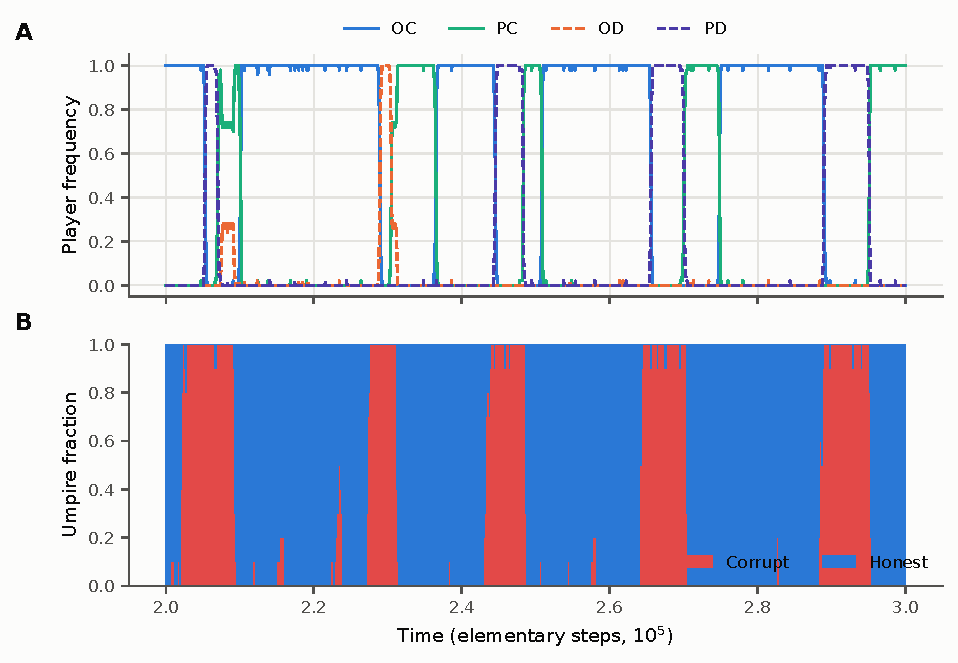
\includegraphics[width=0.78\textwidth]{fig01_small_cycles.pdf}
\caption{Sustained cycles in the small population (reproduction of Lee et al.\ Fig.~1A, B).
(A) Frequencies of OC, PC, OD, and PD. (B) Shares of honest (blue) and corrupt (red) umpires.
One replicate, elementary steps $2$--$3\times10^5$. Parameters: $b=1$, $c=0.5$, $f=B=0.2$,
$h=0.1$, $A=2$, $M=\MSmall$, $N=\NSmall$, $\mu=0.001$, $\nu=0.005$, $s=10^{10}$.}
\label{fig:cycles}
\end{figure*}

\begin{figure}[!t]
\centering
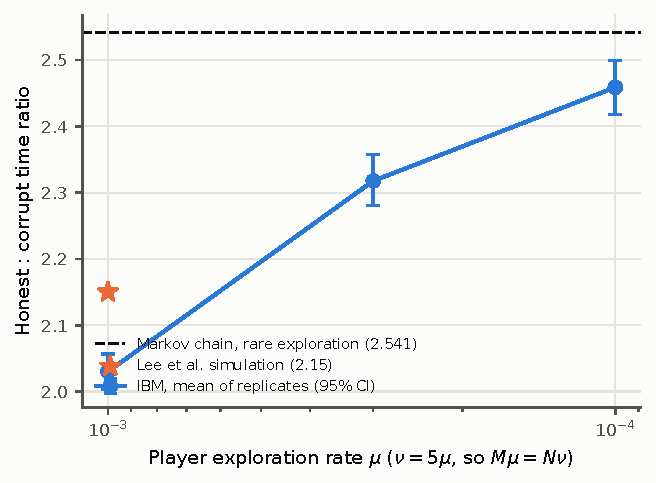
\includegraphics[width=\columnwidth]{fig03_hc_ratio.pdf}
\caption{Honest-to-corrupt time ratio in the small population. Dots: mean over \Nreps{}
replicates with 95\% bootstrap intervals; each replicate runs \BthreeGens{} generations at
$\mu=10^{-3}$ and proportionally longer at smaller $\mu$, with $\nu=5\mu$ so that $M\mu=N\nu$.
Dashed line: rare-exploration Markov chain. Star: value reported by Lee et al.}
\label{fig:ratio}
\end{figure}

In the large population, the simulations follow the exact mean field of the process and settle
at a corrupt fraction of \BfourCorrupt{} after damped oscillations (Fig.~\ref{fig:damped}A). The
mean-field equilibrium is a stable focus with eigenvalues $\FermiRe\pm\FermiIm i$, which
corresponds to a period of about \FermiPer{} generations and a decay time of \FermiDecay{}
generations. In the replicator-mutator equations, raising the exploration rate shrinks the limit
cycle until it disappears in a Hopf bifurcation (Fig.~\ref{fig:damped}B, C). The time series in
Lee et al.'s Fig.~3C, D match the orbit at $\mu=\nu=0.02$ (period \PerViolet; peaks of OC, PC, PD,
and OD \VioletOC, \VioletPC, \VioletPD, and \VioletOD) rather than the orbit at $10^{-4}$ named in
the caption, whose period is \PerSlow{} (Fig.~\ref{fig:damped}D). All discrepancies are listed in
Appendix~\ref{app:typos}.

\begin{figure*}[!t]
\centering
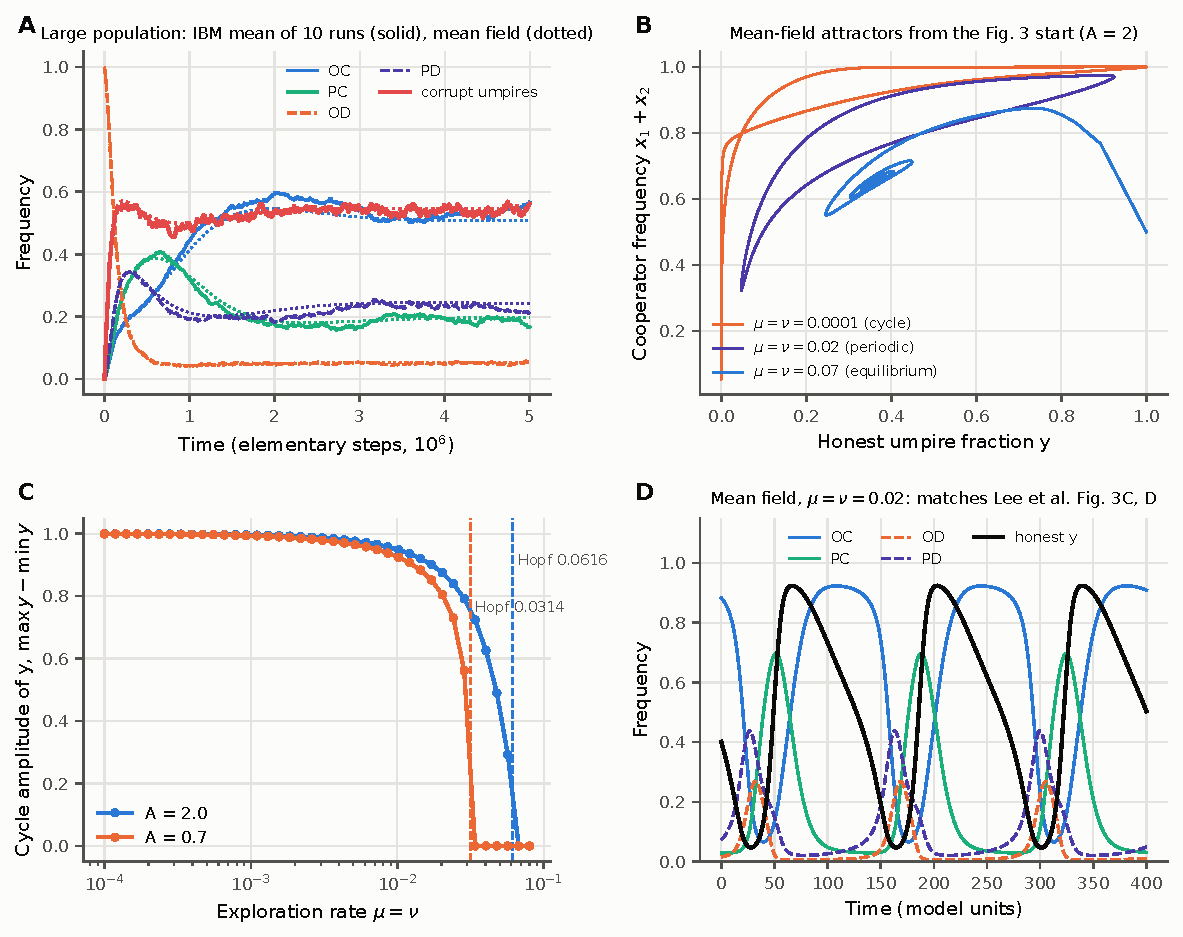
\includegraphics[width=0.8\textwidth]{fig02_damped_and_shrinkage.pdf}
\caption{Damped oscillations and orbit shrinkage. (A) Large population ($M=5000$, $N=1000$,
$\mu=0.01$, $\nu=0.05$, $s=0.3$), start with all OD and all honest umpires: mean of
\LargeReps{} replicates (solid) and exact mean field (dotted). (B) Mean-field attractors in the
plane of honest fraction and cooperator share for $\mu=\nu\in\{10^{-4},0.02,0.07\}$, $A=2$.
(C) Cycle amplitude of $y$ against $\mu=\nu$; dashed lines mark the Hopf points. (D) Mean-field
time series at $\mu=\nu=0.02$, $A=2$, which match Lee et al.'s Fig.~3C, D.}
\label{fig:damped}
\end{figure*}

\subsection{Analytical Results for Rotation}\label{sec:analytic}

\subsubsection{Rotation removes cycles through a SNIC}
Fig.~\ref{fig:bif}A shows the equilibria of the mean field with fresh-cohort rotation (V0,
$p_0=1$) as a function of $\rho$. Without rotation, the only interior equilibrium is an unstable
focus surrounded by the corruption cycle. At $\rhoc=\RhoC$ a fold creates a stable node close to
the all-OC state (honest fraction \FoldY, OC \FoldOC, PC \FoldPC) together with a saddle. The
fold lies on the limit cycle: as $\rho\to\rhoc$ the orbit lingers near the coming equilibrium and
the period grows as $(\rhoc-\rho)^{\alpha}$ with fitted $\alpha=\SnicSlope$, close to the value
$-1/2$ that is characteristic of a saddle-node on an invariant circle (SNIC;
Fig.~\ref{fig:bif}B)~\cite{kuznetsov2004bifurcation}. For $\rho>\rhoc$ all three initial states
we tried went to the honest equilibrium. The unstable focus is destroyed in a second fold at
$\rho=\RhoFtwo$. At the default exploration rate there is no Hopf bifurcation in $\rho$.

\begin{figure*}[!t]
\centering
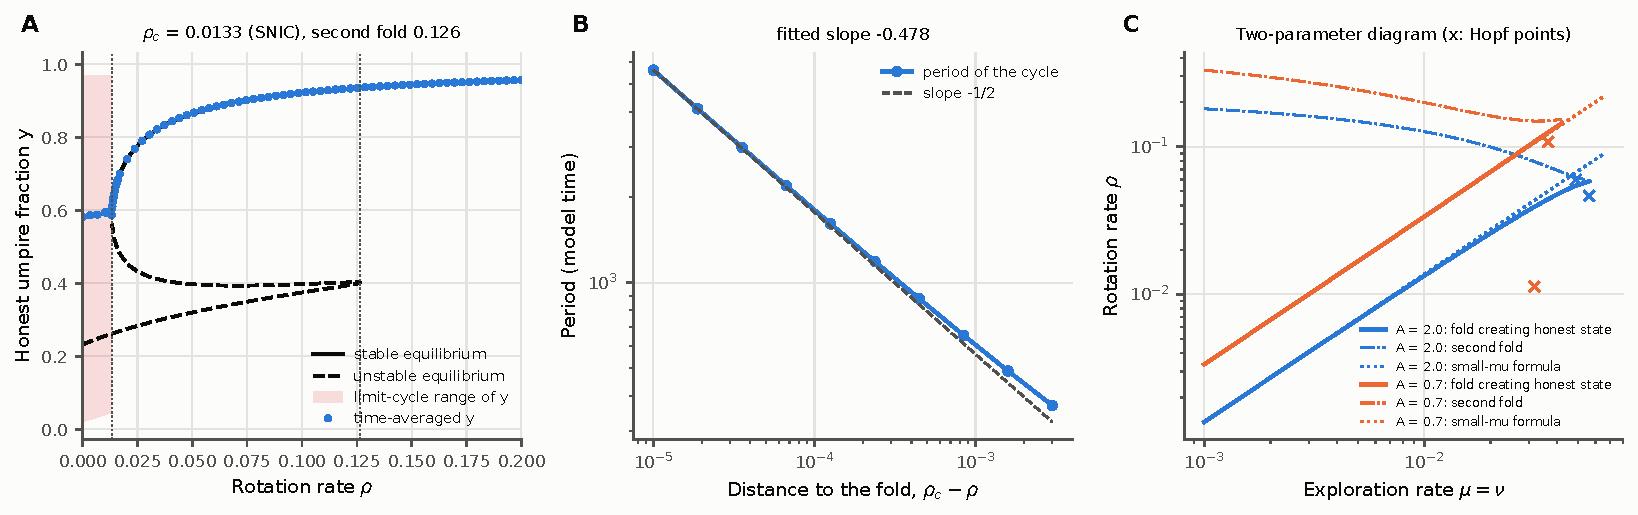
\includegraphics[width=\textwidth]{fig04_bifurcation_rho.pdf}
\caption{Mean-field bifurcations in the rotation rate (V0, $p_0=1$). (A) Honest fraction at the
equilibria (solid stable, dashed unstable), range of $y$ on the limit cycle (shaded), and
time-averaged $y$ (dots); dotted lines mark the folds. $\mu=\nu=\MuMF$, $A=2$. (B) Period of the
cycle against the distance to the fold, log-log; dashed line slope $-1/2$. (C) Fold points
(solid: the fold creating the honest state; dash-dot: the second fold), the small-exploration
formula (dotted), and Hopf points (crosses) as functions of $\mu=\nu$, for $A=2$ and $A=0.7$.}
\label{fig:bif}
\end{figure*}

\subsubsection{An approximation for the critical rotation rate}
Near the all-OC state with small exploration, each rare strategy $j$ is kept at a
mutation-selection balance $x_j\approx\mu/(3d_j(y))$, where $d_j(y)$ is its payoff deficit
against OC:
\begin{align}
d_{\rm PC}&=(1-y)(b-c-f)+h,\nonumber\\
d_{\rm OD}&=y(A-B)-(c-B),\\
d_{\rm PD}&=y(b-f-B)-(c-B-h).\nonumber
\end{align}
OD and PD can invade the OC state when $y$ falls below $y_{\rm OD}=(c-B)/(A-B)$ or
$y_{\rm PD}=(c-B-h)/(b-f-B)$; these are the two ratios compared in the caption of Lee et al.'s
Fig.~3. Inserting $x_j$ into (\ref{eq:ump}) gives $P_H-P_C\approx 4f(x_2-x_4)-2B(x_3+x_4)$, and
the umpire equation (\ref{eq:rot}) has an equilibrium at $y$ when
\begin{equation}
\rho=G(y)=-\frac{y(1-y)\,[P_H-P_C](y)+\nu(1-2y)}{p_0-y}.\label{eq:G}
\end{equation}
The honest equilibrium appears at $\rhoc\approx\min_{y>y_{\rm th}}G(y)$ with
$y_{\rm th}=\max(y_{\rm OD},y_{\rm PD})$. At the default parameters this gives \RhoCApprox{}
(exact \RhoC; error \RhoCErr\%). Because $G$ is linear in $(\mu,\nu)$, the critical rate is
proportional to the exploration rate: $\rhoc/\mu\approx\RhoCOverMuA$ for $A=2$ and \RhoCOverMuB{}
for $A=0.7$ when $\mu=\nu$ (Fig.~\ref{fig:bif}C). For $\mu\le0.011$ the formula is within
\ApproxErrMaxA\% of continuation for $A=2$. For $A=2$ the two folds exist up to
$\mu=\nu\approx\MuMaxFoldA$. Close to the base Hopf point ($\mu=\nu=\HopfMuA$), Hopf points also
appear on the equilibrium branch (crosses in Fig.~\ref{fig:bif}C), so there the route by which
rotation removes the cycle changes; we did not analyze this region in detail.

\subsubsection{Linear inheritance equals slower rotation}
For V1 the whole mean-field system equals the V0 system with $\rho$ replaced by $\rho(1-\kappa)$
(checked symbolically). Every bifurcation point of V0 at $\rho_*$ therefore appears in V1 at
$\rho_*/(1-\kappa)$, which we confirmed by continuation for both folds. The same identity holds
for the pulse map, $(1-\tau)y+\tau[(1-\kappa)p_0+\kappa y]=y+\tau(1-\kappa)(p_0-y)$.

\subsubsection{Dependence on the information cost}
The critical rotation rate depends on $h$ non-monotonically (Fig.~\ref{fig:rhoh}A, B): it peaks at
\RhoCMax{} near $h=\RhoCMaxH$ and falls to \RhoCHighH{} at $h=0.28$. The reason is that
$y_{\rm PD}$ decreases with $h$: when information is costly, prudent defection is less
attractive, and a smaller push toward honesty keeps the OC state safe.

\subsection{Hypotheses}\label{sec:hyp}

Table~\ref{tab:hyp} summarizes the outcomes, which were decided by the pre-registered rules.

\begin{table*}[!t]
\centering
\caption{Outcomes of the Pre-Registered Hypotheses (MF: Mean Field; IBM: Finite Population)}
\label{tab:hyp}
\begin{tabular}{>{\raggedright}p{4.6cm}>{\raggedright}p{2.8cm}>{\raggedright\arraybackslash}p{8.4cm}}
\toprule
Hypothesis & Outcome & Main evidence \\
\midrule
H1: rotation raises honesty, damps cycles & \OutcomeOne & MF: cycles vanish at $\rhoc$; IBM: $\bar y$ \HoneYSZero$\to$\HoneYSMax, episodes \HoneEpSZero$\to$\HoneEpSMax{} per 1000 generations \\
H2: vigilance paradox & \OutcomeTwo & PC \HtwoPCSZero$\to$\HtwoPCSThirty, but episodes shallower (lowest cooperation \HtwoDCSZero$\to$\HtwoDCSTen) and shorter \\
H3: inheritance weakens rotation & \OutcomeThree & Honesty falls with $\kappa$ for V1, V2, V3 in MF and IBM \\
H4: rotation vs.\ transparency & substitutes & Gain from rotation rises with $h$ in \HfourInc{} of \HfourPairs{} MF pairs and \HfourIncIBM{} of \HfourPairsIBM{} IBM pairs \\
H5: conformist bistability & \OutcomeFive & Bistable only for $\kappa\ge\HfiveKminDefault$; no loop in the pre-registered sweep \\
H6: delay destabilizes & \OutcomeSix & Rightmost root $\le\HsixMaxRe$ at all \HsixPoints{} points \\
\bottomrule
\end{tabular}
\end{table*}

\subsubsection{H1: rotation raises honesty and damps cycles (\OutcomeOne)}
In the mean field the amplitude of the cycle is unchanged until $\rhoc$ and zero beyond it
(Fig.~\ref{fig:bif}A). Time-averaged honesty is nearly flat below $\rhoc$ (\YbarZero{} at
$\rho=0$, \YbarLastCycle{} just below $\rhoc$) because the orbit spends more time near the ghost
of the coming equilibrium, then rises to \YbarRhoFive{} at $\rho=0.05$ and \YbarRhoTwenty{} at
$\rho=0.2$. In the small finite population, honesty rises from \HoneYSZero{} [\HoneYSZeroLo,
\HoneYSZeroHi] without rotation to \HoneYSMax{} [\HoneYSMaxLo, \HoneYSMaxHi] at
$\rho=\HoneRhoMaxIBM$ per generation, and corruption episodes fall from \HoneEpSZero{} to
\HoneEpSMax{} per 1000 generations (Fig.~\ref{fig:h2}D, F). In the large population honesty rises
from \HoneYLZero{} to \HoneYLMax{}, and episodes with $y<0.5$ disappear for $\rho\ge0.05$. There,
the time-averaged honesty with rotation is within \NeutralMaxDev{} of $(\nu+\rho)/(2\nu+\rho)$,
the value expected if selection between umpire types were neutral, for all $\rho\ge0.05$.

\begin{figure*}[!t]
\centering
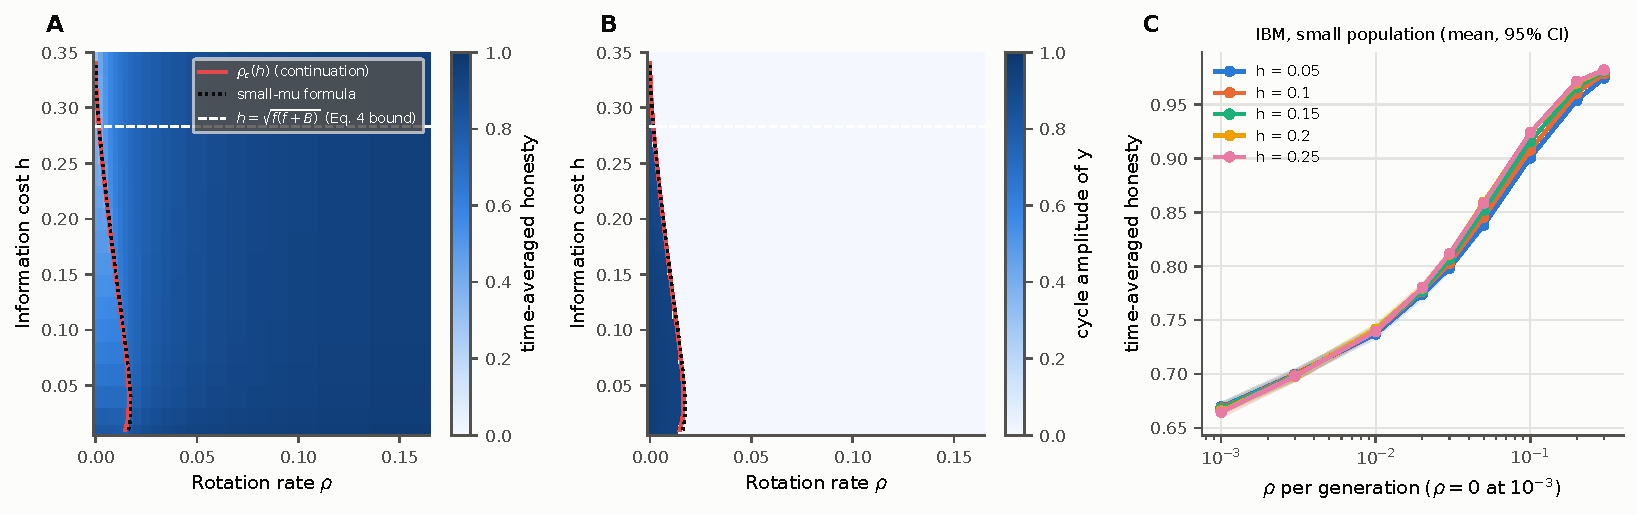
\includegraphics[width=\textwidth]{fig05_rho_h.pdf}
\caption{Rotation and the information cost $h$ (V0, $p_0=1$). (A) Mean-field time-averaged
honesty; red line: critical rate $\rhoc(h)$ from continuation; dotted: small-exploration formula;
dashed white: the bound $h=\sqrt{f(f+B)}$ of Lee et al. (B) Mean-field cycle amplitude of $y$.
$\mu=\nu=\MuMF$, burn-in \TBurnMF, window \TWinMF. (C) Small finite population: mean honesty with
95\% bootstrap bands over \Nreps{} replicates of \WinSmall{} generations; $\rho=0$ is plotted at
$10^{-3}$.}
\label{fig:rhoh}
\end{figure*}

\subsubsection{H2: the vigilance paradox (\OutcomeTwo)}
Rotation lowers vigilance as predicted. In the small population the frequency of prudent
cooperators falls from \HtwoPCSZero{} to \HtwoPCSTen{} at $\rho=0.1$ and \HtwoPCSThirty{} at
$\rho=0.3$; in the mean field from \PCZero{} to \PCLastCycle{} just below $\rhoc$ and \PCFirstEq{}
at the honest equilibrium. But the remaining episodes are not deeper (Fig.~\ref{fig:h2}). In the
small population the lowest cooperator share during an episode rises from \HtwoDCSZero{}
[\HtwoDCSZeroLo, \HtwoDCSZeroHi] to \HtwoDCSTen{} [\HtwoDCSTenLo, \HtwoDCSTenHi] at $\rho=0.1$,
peak corruption falls from \HtwoDYSZero{} to \HtwoDYSTen{}, and episodes last \HtwoRecSZero{}
generations without rotation and \HtwoRecSThirty{} at $\rho=0.3$. In the mean field, peak
corruption falls from \DepthYZero{} to \DepthYLast{} and the lowest cooperator share rises from
\DepthCZero{} to \DepthCLast{} as $\rho$ approaches $\rhoc$. A likely reason why fewer prudent
players do not lead to worse episodes is that rotation also feeds honest umpires into the episodes
themselves, which shortens them before cooperation collapses fully; we did not test this mechanism
directly.

\begin{figure*}[!t]
\centering
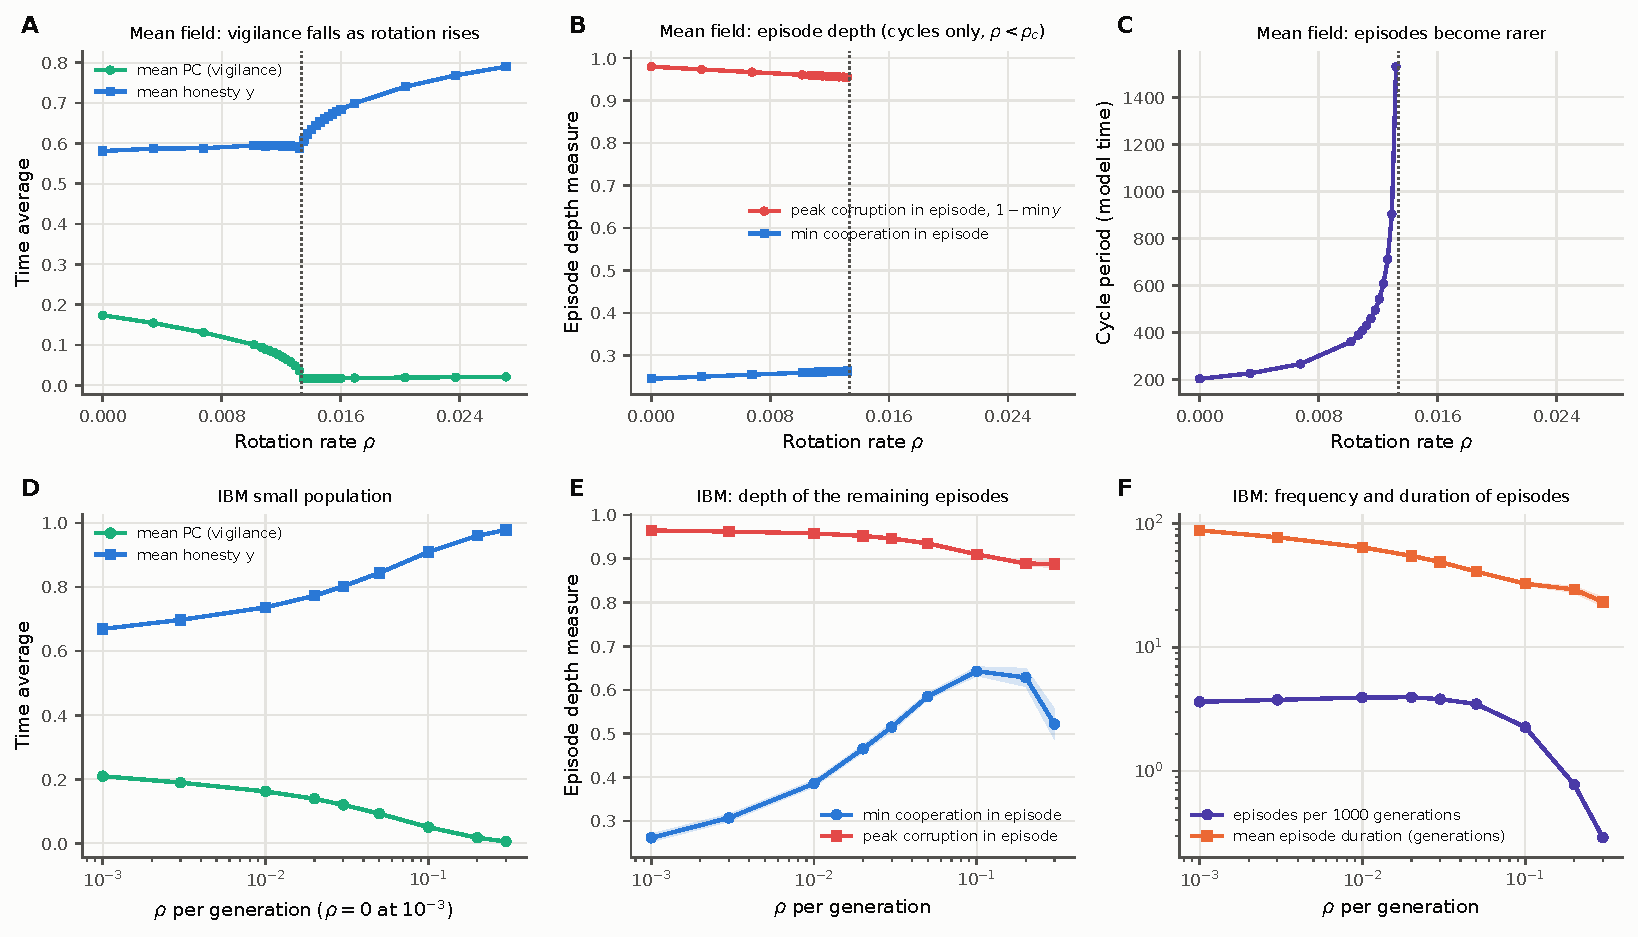
\includegraphics[width=\textwidth]{fig07_vigilance_h2.pdf}
\caption{Vigilance and the depth of corruption episodes (V0, $p_0=1$). Top: mean field
($\mu=\nu=\MuMF$, $A=2$); dotted line marks $\rhoc$; depth and period are shown only where a cycle
exists. Bottom: small finite population, means with 95\% bootstrap bands over \Nreps{} replicates
of \WinSmall{} generations. An episode is a maximal interval with $y<0.5$; in the finite
population, gaps shorter than 5 generations are merged and episodes shorter than 5 generations
are dropped.}
\label{fig:h2}
\end{figure*}

\subsubsection{H3: inheritance weakens rotation (\OutcomeThree)}
In the mean field, honesty falls with $\kappa$ at every rotation rate for V1 and V3 and at most
rates for V2, and the region without cycles shrinks (Fig.~\ref{fig:kappa}A--C). For V1 the
boundary is exactly $\rho(1-\kappa)=\rhoc$. V2 weakens rotation least, because at the honest
equilibrium $y>1/2$ and conformity then favors honesty. In the small population, honesty falls
with $\kappa$ for all three variants at all three rotation rates tested
(Fig.~\ref{fig:kappa}D--F). The finite-population test of the V1 equivalence compares V1 at
$(\rho,\kappa)$ with V0 at $\rho(1-\kappa)$; the difference in mean honesty was at most
\HthreeMaxDiff, but its 95\% interval excluded zero at \HthreeNexcl{} of \HthreeNtests{} points.
By the pre-registered rule the equivalence therefore does not hold exactly in the finite
population; with a Bonferroni adjustment for \HthreeNtests{} comparisons (a post-hoc check) it
\HthreeBonf.

\begin{figure*}[!t]
\centering
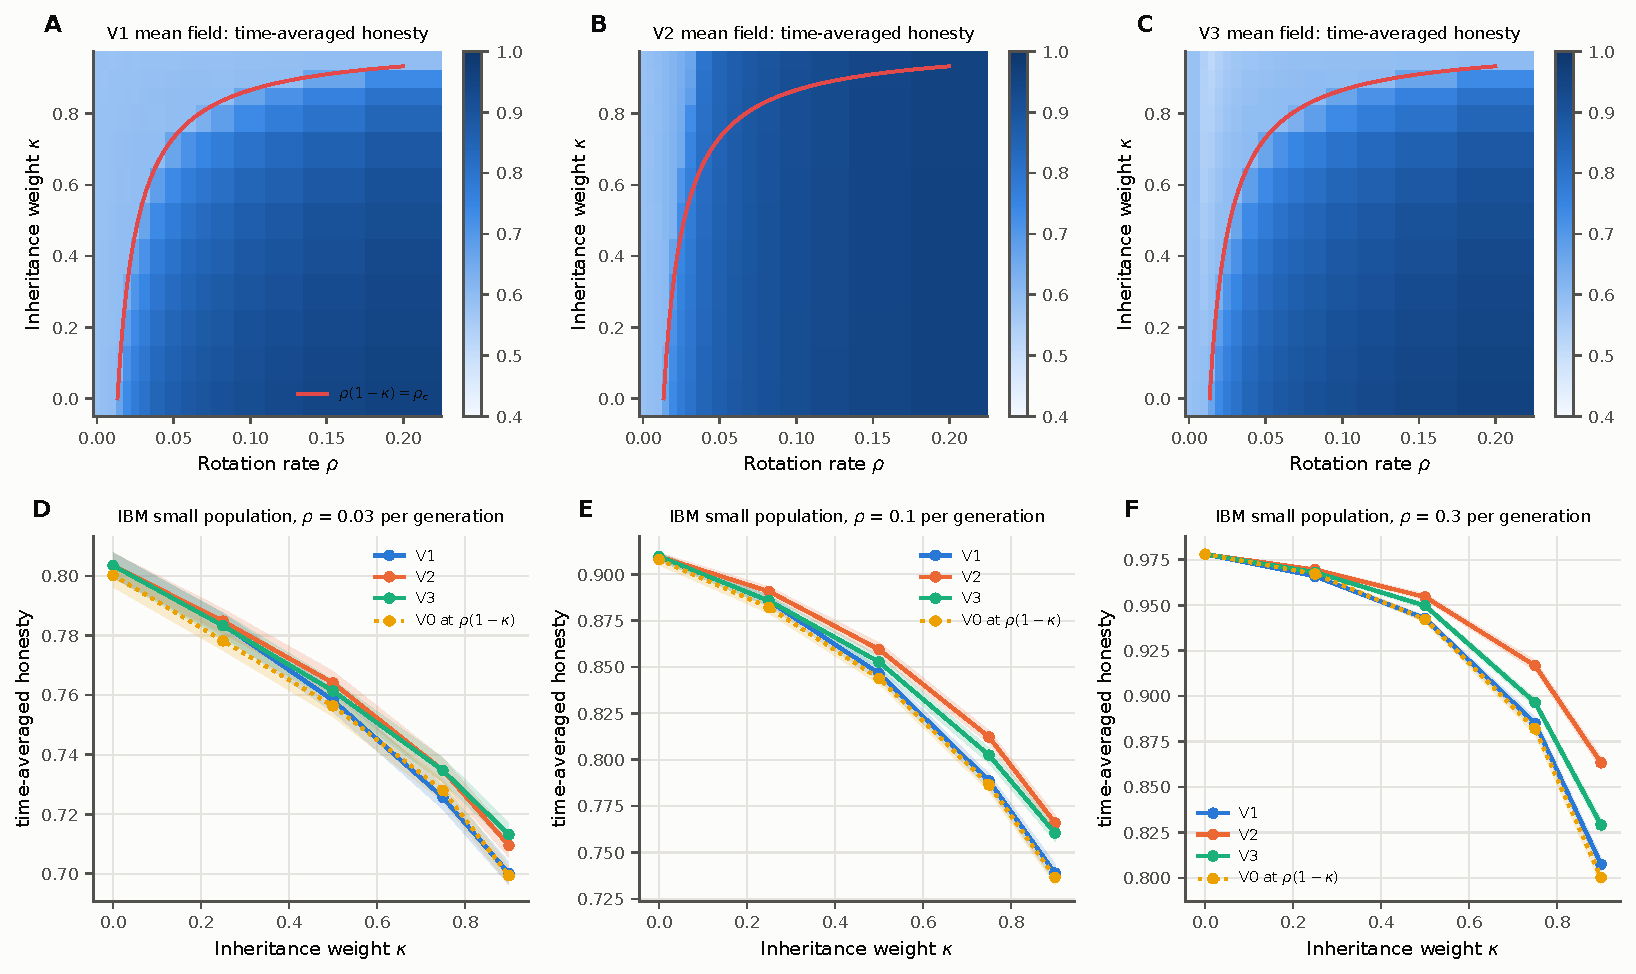
\includegraphics[width=\textwidth]{fig06_rho_kappa.pdf}
\caption{Inherited integrity. (A)--(C) Mean-field time-averaged honesty for V1, V2 ($k=2$), and
V3 ($T_{\rm lag}=1/\rho$) over rotation rate and inheritance weight; red line:
$\rho(1-\kappa)=\rhoc$. $\mu=\nu=\MuMF$. (D)--(F) Small finite population at $\rho=0.03$, $0.1$,
and $0.3$ per generation: mean honesty with 95\% bootstrap bands over \Nreps{} replicates; dotted:
fresh rotation at $\rho(1-\kappa)$.}
\label{fig:kappa}
\end{figure*}

\subsubsection{H4: rotation and transparency are substitutes}
If rotation helps more where information is costly, the two act as substitutes. In the mean field
the gain in honesty from rotation increased with $h$ for \HfourInc{} of \HfourPairs{} neighboring
pairs in the admissible range of $h$ (for example \GainLowH{} at $h=0.02$ and \GainHighH{} at
$h=0.28$ for $\rho=0.05$), so the pre-registered rule classifies them as substitutes for honesty.
For the cooperator share the pattern is mixed (\HfourIncC{} pairs increasing, \HfourDecC{}
decreasing). In the small population the gain increased with $h$ in \HfourIncIBM{} of
\HfourPairsIBM{} pairs, while honesty without rotation hardly depended on $h$ (\HfourYZeroMin{} to
\HfourYZeroMax), as the rare-exploration result of Lee et al.\ predicts (Fig.~\ref{fig:rhoh}C).

\subsubsection{H5: conformist inheritance and bistability (\OutcomeFive)}
In the pre-registered scan over $h$, exploration rate, conformity exponent, $\kappa$, and $\rho$,
only \HfiveNbi{} of \HfiveNscan{} points showed different attractors from an honest and a corrupt
start, and the pre-registered sweeps of $\kappa$ showed no loop (largest gap \HfiveGapPre;
Fig.~\ref{fig:hyst}A, F). A targeted follow-up found an open bistable region, but only when
newcomers almost purely copy the majority ($\kappa\ge\HfiveKminDefault$ at default parameters,
$\kappa\ge\HfiveKminStrong$ with $h=0.29$ and $k=4$) and rotation is fast (Fig.~\ref{fig:hyst}B,
C). A post-hoc sweep that starts from the corrupt state shows hysteresis (gap \HfiveGapPost;
Fig.~\ref{fig:hyst}D). In the finite population the time-averaged honesty did not depend on the
starting state at these points, for $N=10$ and $N=100$ (Fig.~\ref{fig:hyst}E), so noise switches
between the two states. The hypothesis is therefore only partly supported.

\begin{figure*}[!t]
\centering
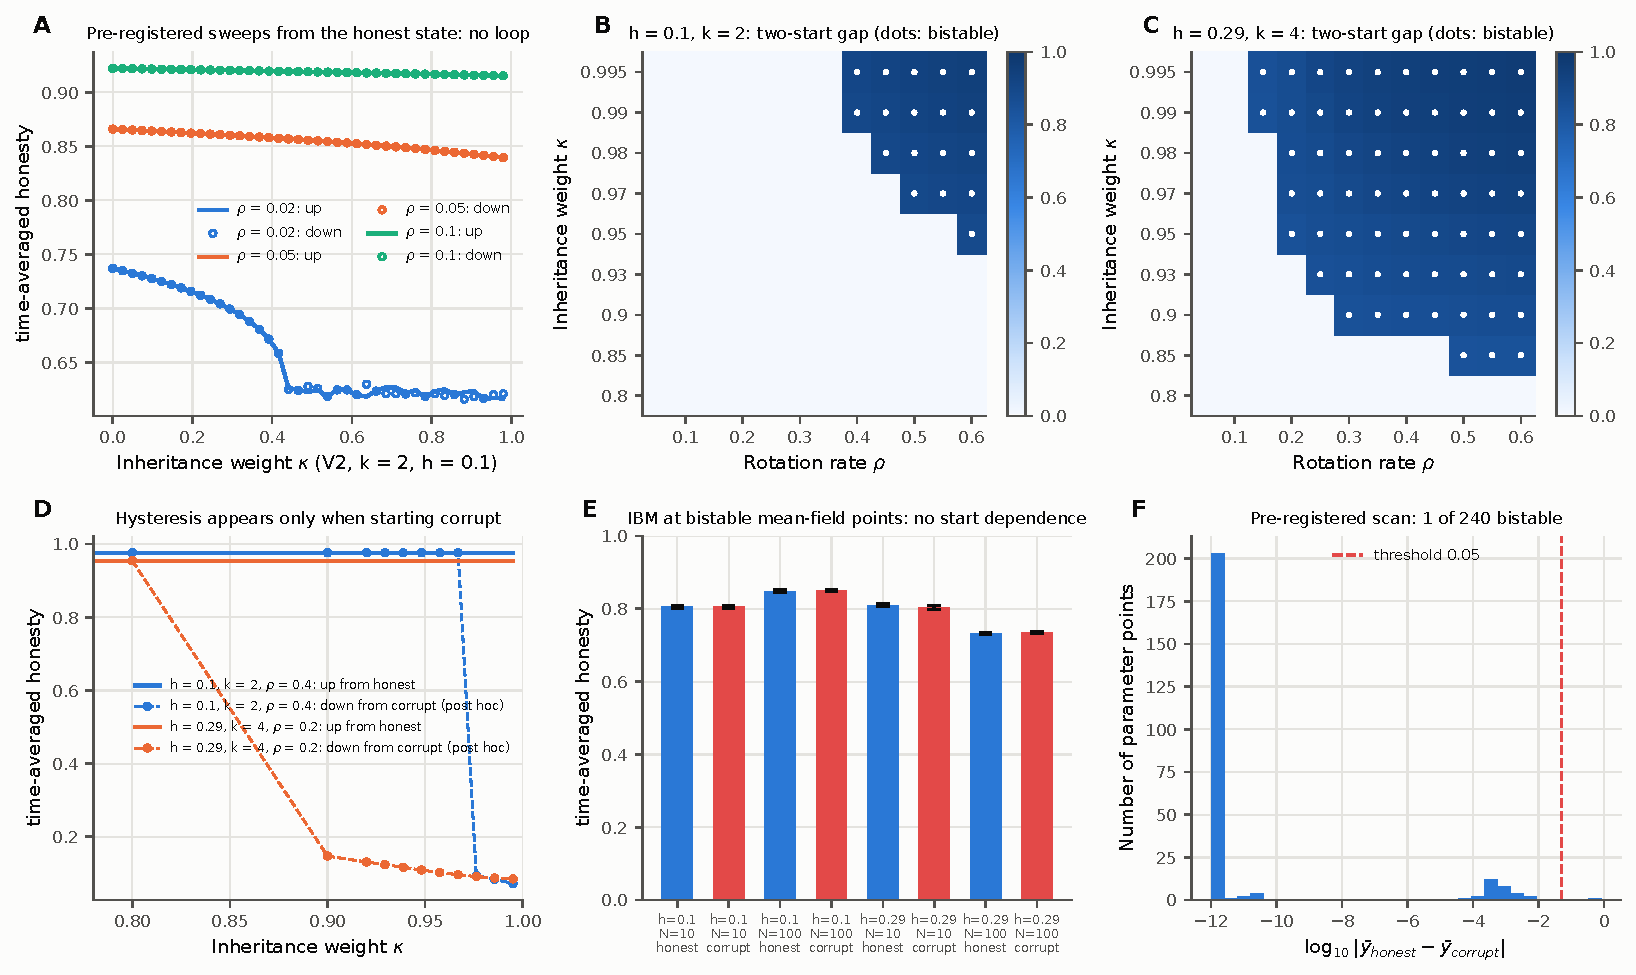
\includegraphics[width=\textwidth]{fig08_conformist_hysteresis.pdf}
\caption{Conformist inheritance (V2). (A) Pre-registered sweeps of $\kappa$ up and down,
continuing the state, at three $\rho$ ($h=0.1$, $k=2$, $\mu=\nu=\MuMF$). (B), (C) Difference in
time-averaged honesty between honest and corrupt starts over $(\rho,\kappa)$; dots mark points
where it exceeds 0.05. (D) Sweeps up from the honest state and down from the corrupt state
(post hoc). (E) Small and medium finite populations at bistable mean-field points, honest and
corrupt starts, means with 95\% intervals over \Nreps{} replicates. (F) Distribution of the
two-start difference in the pre-registered scan (log scale).}
\label{fig:hyst}
\end{figure*}

\subsubsection{H6: delayed inheritance (\OutcomeSix)}
The equilibria of V3 are those of V1, so the honest equilibrium exists when
$\rho(1-\kappa)>\rhoc$. Delay could in principle destabilize it. Across \HsixPoints{}
combinations of $\rho\in\{0.05,0.1,0.2\}$, $\kappa$, and $T_{\rm lag}$ from 0 to 400, the
rightmost characteristic root had real part at most $\HsixMaxRe$, and a check with twice the
collocation nodes gave the same picture (Fig.~\ref{fig:delay}). Longer delays only slowed the
return to the honest state. Direct simulations of the delay equation agreed.

\begin{figure*}[!t]
\centering
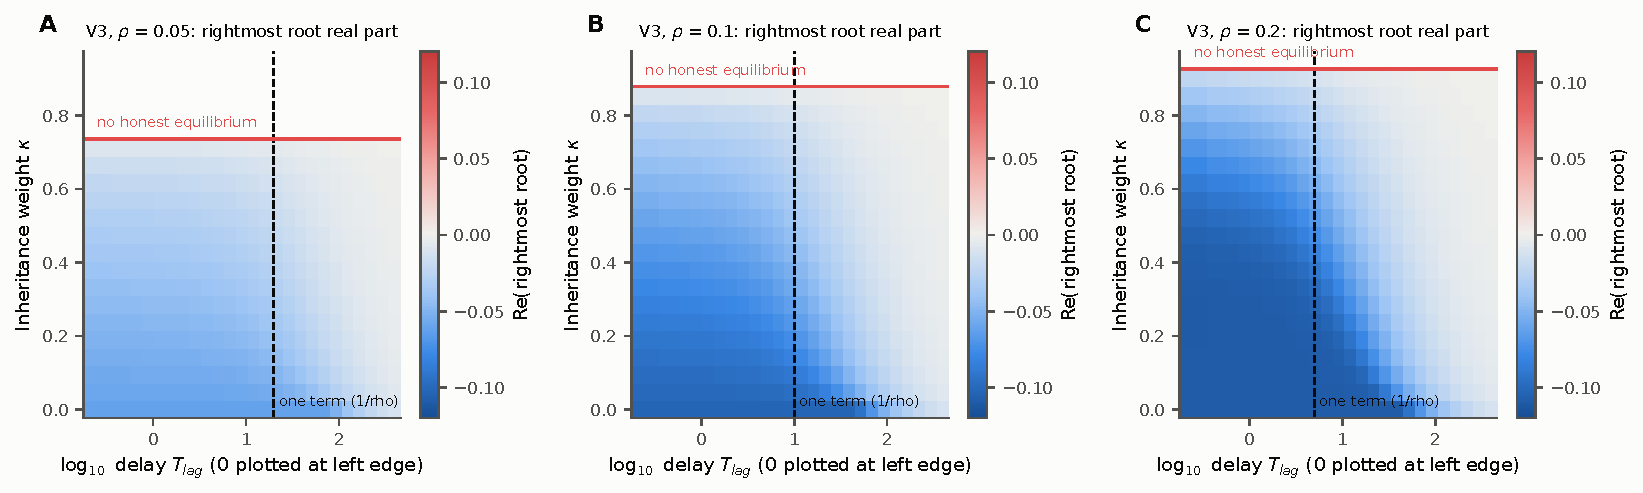
\includegraphics[width=\textwidth]{fig09_delay_stability.pdf}
\caption{Delayed inheritance (V3). Real part of the rightmost characteristic root of the honest
equilibrium over delay and inheritance weight, for $\rho=0.05$, $0.1$, and $0.2$
($\mu=\nu=\MuMF$). Blue: stable. Dashed line: one term, $T_{\rm lag}=1/\rho$. Above the red line
no honest equilibrium exists ($\rho(1-\kappa)<\rhoc$).}
\label{fig:delay}
\end{figure*}

\subsection{Robustness}

Replacing whole cohorts at once is more effective than gradual replacement at the same average
rate. In the mean field at $\rho=0.02$, continuous rotation gives honesty \PulseMFCont{} and
replacing all umpires every $1/\rho$ time units gives \PulseMFFull. In the small population at
$\rho=0.03$ the values are \PulseIBMCont{} [\PulseIBMContLo, \PulseIBMContHi] and
\PulseIBMFull{} [\PulseIBMFullLo, \PulseIBMFullHi] (Fig.~\ref{fig:S3}). When newcomers are not
reliably honest, rotation needs to be faster and can backfire: $\rhoc$ rises to
\RhoCpZeroNinety, \RhoCpZeroSeventyFive, and \RhoCpZeroSixty{} for $p_0=0.9$, $0.75$, and $0.6$,
and with $p_0=0.6$ moderate rotation lowers honesty to \PZeroSixtyMin. With a smaller fine
($A=0.7$) the equilibrium curve has the same two folds and no Hopf point, with $\rhoc=\RhoCAseven$.
In one-at-a-time variations of $\pm20\%$ that respect the parameter conditions, $\rhoc$ ranged
from \OATRhoCMin{} to \OATRhoCMax{} and honesty at $\rho=\RhoProbe$ from \OATProbeMin{} to
\OATProbeMax{} (Fig.~\ref{fig:S2}). Rotation raised honesty at all population sizes tested
(Fig.~\ref{fig:val}B); larger populations had lower honesty without rotation (\FinSmallZero{} for
$M=50$, \FinLargeZero{} for $M=\FinMmax$) and needed faster rotation for the same effect.

\begin{figure*}[!t]
\centering
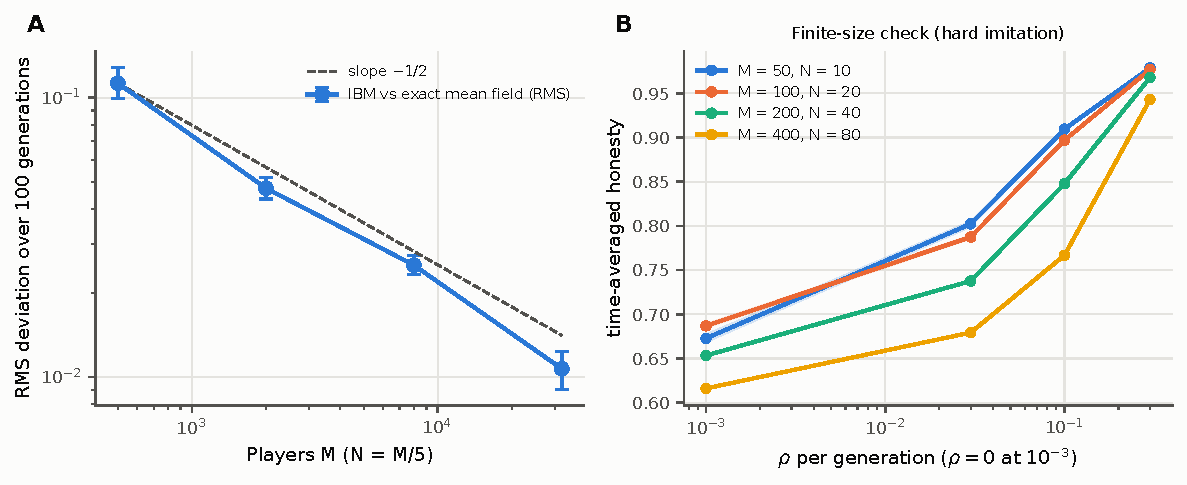
\includegraphics[width=0.75\textwidth]{fig10_validation_finite_size.pdf}
\caption{Validation and finite size. (A) Root-mean-square deviation between the finite
population and its exact mean field over 100 generations, against $M$ ($N=M/5$, large-population
rates, 8 replicates, 95\% intervals); dashed: slope $-1/2$. (B) Mean honesty against rotation rate
for $M\in\{50,100,200,400\}$, $N=M/5$, small-population rates, \Nreps{} replicates, 95\% bands.}
\label{fig:val}
\end{figure*}

%=====================================================================
\section{Discussion}
%=====================================================================

\subsection{Interpretation}
Lee et al.\ showed that institutional corruption need not settle at a fixed level: when watching
the watchers is costly, honesty and corruption chase each other in cycles~\cite{lee2019social}. We
asked what term limits do to this cycle. In the model, regular replacement of umpires by honest
newcomers removes the cycle once the replacement rate passes a critical value. Below that value
the cycle survives but slows down, and the average level of honesty barely changes. Above it the
institution settles in a state where nearly all players cooperate optimistically and few check
their umpires. The transition is a saddle-node on the cycle rather than a Hopf bifurcation, which
has a practical reading: the system does not move smoothly from small oscillations to stability.
Instead, corruption episodes become rarer and rarer as the rotation rate rises and then stop. The
critical rate is proportional to how often umpires explore corrupt behavior, so the model says
that the turnover needed to keep an institution honest scales with the rate at which its members
are tempted to try corruption.

The vigilance paradox we expected did not appear. Rotation did make players less vigilant, but
the episodes of corruption that remained were milder and shorter. Within this model, then, the
loss of vigilance is not dangerous as long as the supply of honest newcomers continues. This
conclusion depends on that supply. When newcomers inherit the integrity of the body they join, the
benefit of rotation shrinks, and linear inheritance is exactly equivalent to slower rotation. When
newcomers are not reliably honest, rotation can even lower honesty. Conformist inheritance can
lock an institution into corruption only in an extreme regime where newcomers almost purely follow
the majority, and this lock-in did not survive noise in our finite-population simulations.

\subsection{Model Implications for Real Institutions}
These results suggest implications for real institutions, stated here as model implications and
not as empirical claims. First, the value of term limits depends on what newcomers bring:
training or selection that makes newcomers reliably honest matters as much as the rotation rate.
Second, mentoring by incumbents transmits whatever the incumbents are, so in a body with a corrupt
majority it works against rotation. Third, replacing whole cohorts at once, as in annual elections
of an entire board, was more effective in the model than staggered replacement at the same
average rate. Student organizations, where leadership often changes every year, are a natural
setting in which these predictions could be examined; the experience of the author with the
regulations governing such organizations at ITB motivated this question, but the model has not
been tested against data from them.

\subsection{Relation to Prior Work}
Enforcer ``education'' that raises the trial rate of honest conduct curbs corruption in a model of
illegal logging~\cite{lee2015logging}, and higher exploration rates of enforcers reduce corruption
in a model with optional external supervision~\cite{zhou2023supervision}. In the mean field,
fresh-cohort rotation is formally the same mechanism; our contribution is the bifurcation
structure, the inheritance variants, and the finite-population analysis. Staff rotation has been
tested as an anti-corruption policy in laboratory
experiments~\cite{abbink2004rotation,buhren2020rotation}, and empirical studies relate corruption
to term limits and re-election incentives~\cite{ferraz2011electoral,laurent2021horizon}. Our
model omits elections and reputation, so it does not speak to those incentive effects.

\subsection{Limitations}
The supplementary information of Lee et al.\ was not available, so our individual-based update
rule is a reconstruction; it reproduces the published figures closely but gives a lower
honest-to-corrupt ratio (\BthreeRatio{} against \PaperRatio). The rotation rate is measured in
model time in the mean field and in generations in the simulations, and these units are not
directly comparable because hard imitation is not the weak-selection limit. Populations are well
mixed; players and umpires learn at the same per-capita rate; the inheritance rules are our own
simple choices; and the game involves two players. The mean-field default exploration rate
(\MuMF) is higher than the orange orbit of Lee et al.\ ($10^{-4}$); we checked $10^{-3}$ and
$0.02$ and found the same picture with $\rhoc$ proportional to $\mu$.

\subsection{Future Work}
Several extensions would be natural: a formal asymptotic derivation of $\rhoc$; heterogeneous
term lengths; mentoring on networks rather than in a well-mixed body; elections in which players
choose umpires; and an analysis of pulsed rotation as a periodically forced system, which could
explain why whole-cohort replacement works better.

%=====================================================================
\section{Conclusion}
%=====================================================================
We reproduced the corruption model of Lee et al.\ from its main text, confirmed its analytical
results exactly, and documented six inconsistencies in the published text. Adding term-limited
umpires showed that rotation with reliably honest newcomers removes corruption cycles through a
saddle-node on the cycle at a critical rate proportional to the exploration rate, raises honesty,
and shortens corruption episodes even as vigilance declines. The benefit depends on what newcomers
learn: inheritance from incumbents weakens it, conformist inheritance can lock in either state only
in an extreme regime, and delayed inheritance does not destabilize the honest state.

\appendices

\section{Derivations}\label{app:deriv}

\subsubsection{Umpire income} With $x$ the strategy frequencies and pairs drawn independently, an
honest umpire earns $2f$ unless a PD is present, so $P_H=2f(1-x_4)^2$. A corrupt umpire earns
nothing if a PC is present; otherwise it earns $2f$ plus $B$ per defector, so
$P_C=2f(1-x_2)^2+2B(x_3+x_4)(1-x_2)$. Using $2-x_2-x_4=1+x_1+x_3$ on the simplex gives
(\ref{eq:ump}). We verified this by enumerating all ordered strategy pairs with a rule-based
implementation of a single game.

\subsubsection{Linear inheritance} $\rho[(1-\kappa)p_0+\kappa y-y]=\rho(1-\kappa)(p_0-y)$, so the
V1 system is the V0 system with $\rho\to\rho(1-\kappa)$; for pulses,
$(1-\tau)y+\tau[(1-\kappa)p_0+\kappa y]=y+\tau(1-\kappa)(p_0-y)$.

\subsubsection{Invasion thresholds} At the OC vertex the payoff of OC is $b-c-f$, that of OD is
$y(b-f-A)+(1-y)(b-f-B)$, and that of PD is $-yh+(1-y)(b-f-B-h)$. OD does better than OC when
$y<y_{\rm OD}=(c-B)/(A-B)$, and PD when $y<y_{\rm PD}=(c-B-h)/(b-f-B)$. At base parameters
$y_{\rm PD}=\yPD$, and $y_{\rm OD}=\yODA$ for $A=2$ and \yODB{} for $A=0.7$. As honesty drifts down
along the OC edge, the strategy with the larger threshold invades first: PD for $A=2$ and OD for
$A=0.7$. This explains which corner the cycle visits.

\subsubsection{Critical rotation rate} For a rare strategy $j$ near the OC vertex,
$\dot x_j\approx -d_j(y)x_j+\mu/3$, so $x_j\approx\mu/(3d_j)$. To first order in $x_j$,
$P_H-P_C=4f(x_2-x_4)-2B(x_3+x_4)$, which gives (\ref{eq:G}). The honest equilibrium exists for
$\rho\ge\min_{y>y_{\rm th}}G(y)$. The approximation requires $d_j\gg\mu$, which fails close to
$y_{\rm th}$, but the minimum lies at $y\approx\RhoCy$, well above the thresholds.

\subsubsection{Neutral umpire selection} If $P_H=P_C$, (\ref{eq:rot}) with $p_0=1$ gives
$\nu(1-2y)+\rho(1-y)=0$, so $y=(\nu+\rho)/(2\nu+\rho)$.

\section{Reproduction Notes and Resolved Typos}\label{app:typos}

\begin{table*}[!t]
\centering
\caption{Discrepancies with Lee et al.\ (2019) and Their Resolution}
\label{tab:typos}
\begin{tabular}{>{\raggedright}p{0.8cm}>{\raggedright}p{2.5cm}>{\raggedright}p{6.0cm}>{\raggedright\arraybackslash}p{6.4cm}}
\toprule
ID & Location & Issue & Resolution \\
\midrule
D1 & Methods & $Q(y)=y_1Q_C+(1-y_1)Q_H$ with $y_1$ the honest fraction & $Q(y)=y_1Q_H+(1-y_1)Q_C$; the printed form fails B1 \\
D2 & Methods & Honest mixed state called ``OD+PD (a mixture of OD and PC)'' & It mixes OD and PD (Fig.~2 caption, $Q_H$) \\
D3 & Fig.~3 caption & ``8 or 9, respectively'' reversed relative to the figure & With $A=2$ the orbit passes state 9, with $A=0.7$ state 8 (Appendix~\ref{app:deriv}) \\
D4 & Transition matrix & Row 3 omits the transition to state 8 & State 3 is transient; no effect \\
D5 & Transition matrix & Row 4 gives $\mu/6$ to a neutral player mutant & State 4 is transient; no effect \\
D6 & Fig.~3C, D & Caption names the $\mu=\nu=10^{-4}$ orbit & Panels match $\mu=\nu=0.02$ \\
U1 & SI (not available) & Individual-based update procedure & Reconstructed: random sequential updates, role model from own population, expected payoffs, time in elementary steps \\
\bottomrule
\end{tabular}
\end{table*}

Table~\ref{tab:typos} lists all discrepancies. The time unit was inferred from Lee et al.'s
Fig.~1: with one individual updating per elementary step, entry rates of new strategies are equal
in both populations when $M\mu=N\nu$, as the caption states, and the number of episodes per
$10^5$ steps matches the figure. All signs of the payoff matrices were read from the PDF at
300~dpi; the PMC web version lost minus signs.

\section{Parameters}\label{app:params}

\begin{table}[!t]
\centering
\caption{Parameter Values}
\label{tab:params}
\begin{tabular}{>{\raggedright}p{2.0cm}>{\raggedright\arraybackslash}p{5.8cm}}
\toprule
Symbol & Value (source) \\
\midrule
$b,c,f,B,h,A$ & $1,\ 0.5,\ 0.2,\ 0.2,\ 0.1,\ 2$, or $A=0.7$ (Lee et al., Figs.~1, 3) \\
Small setting & $M=50$, $N=10$, $\mu=0.001$, $\nu=0.005$, $s=10^{10}$ (Lee et al., Fig.~1A, B) \\
Large setting & $M=5000$, $N=1000$, $\mu=0.01$, $\nu=0.05$, $s=0.3$ (Lee et al., Fig.~1C, D) \\
Mean-field exploration & $\mu=\nu=\MuMF$; also $10^{-3}$, $0.02$ (this work) \\
Rotation & $\rho\in[0,0.2]$ (mean field); $[0,0.3]$ per generation (this work) \\
Inheritance & $\kappa\in[0,0.995]$, $k=2$ (also 4), $p_0=1$ (also 0.9, 0.75, 0.6) (this work) \\
Delay & $T_{\rm lag}=1/\rho$ (default), $0$ to $400$ (this work) \\
\bottomrule
\end{tabular}
\end{table}

Table~\ref{tab:params} lists the parameters. The base mean-field cycle has period about \PerSlow{}
at $\mu=\nu=10^{-4}$, \PerZero{} at $\mu=\nu=\MuMF$, and \PerViolet{} at $0.02$; the Hopf point is
at \HopfMuA.

\section{Numerical and Statistical Checks}\label{app:checks}

Tightening the tolerances tenfold and switching to an explicit Runge-Kutta method changed honesty,
amplitude, and minimum cooperation by at most $\TolMaxDiff$ at 16 test points. On a grid eight
times finer in a sub-region ($\rho$ step \FineGridStep), the first rotation rate with an
equilibrium was within \FineGridMaxOff{} of the continuation value of $\rhoc$. The
finite-population simulation agrees with its exact mean field with an error that decreases as
$M^{-1/2}$ (\ValRmsA{} at $M=\ValMA$, \ValRmsD{} at $M=\ValMD$). With rotation rate set to zero,
the code reproduces the base model bit for bit. Doubling the averaging window left the
honest-to-corrupt ratio unchanged (\BthreeDouble). The test suite checks payoffs against a
rule-based game, the symbolic Jacobian against finite differences, the delay solver against an
exact solution, and the V1 equivalence symbolically.

\section{Literature Search}\label{app:lit}
We searched the web (October 2026) for evolutionary-game models of corruption that include
rotation, term limits, or turnover of enforcers. We found none. The closest work studies enforcer
education~\cite{lee2015logging}, enforcer exploration~\cite{zhou2023supervision}, corrupt
enforcers in pool punishment~\cite{liu2019corrupt}, and supervision of
umpires~\cite{shi2023bidirectional}. Rotation itself has been studied
experimentally~\cite{abbink2004rotation,buhren2020rotation}, and term limits
empirically~\cite{ferraz2011electoral,laurent2021horizon}.

\section{Supplementary Figures}

\begin{figure*}[!t]
\centering
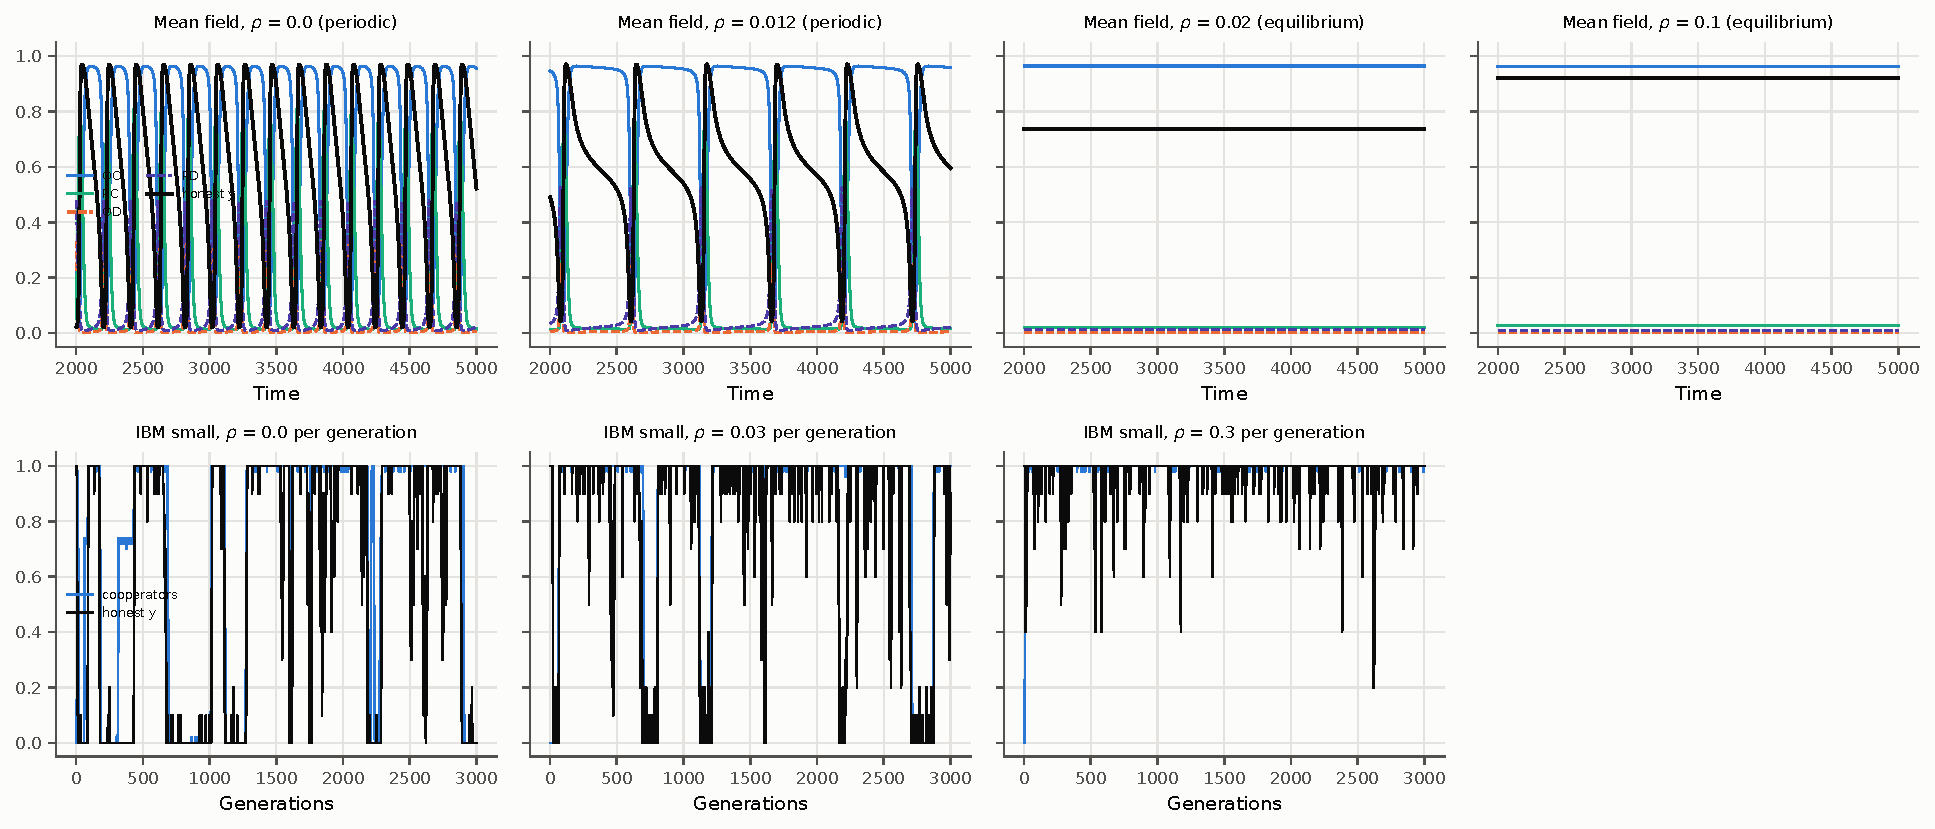
\includegraphics[width=\textwidth]{figS1_time_series.pdf}
\caption{Time series. Top: mean field at $\rho=0$, $0.012$, $0.02$, and $0.1$ ($\mu=\nu=\MuMF$).
Bottom: one small-population replicate at $\rho=0$, $0.03$, and $0.3$ per generation.}
\label{fig:S1}
\end{figure*}

\begin{figure*}[!t]
\centering
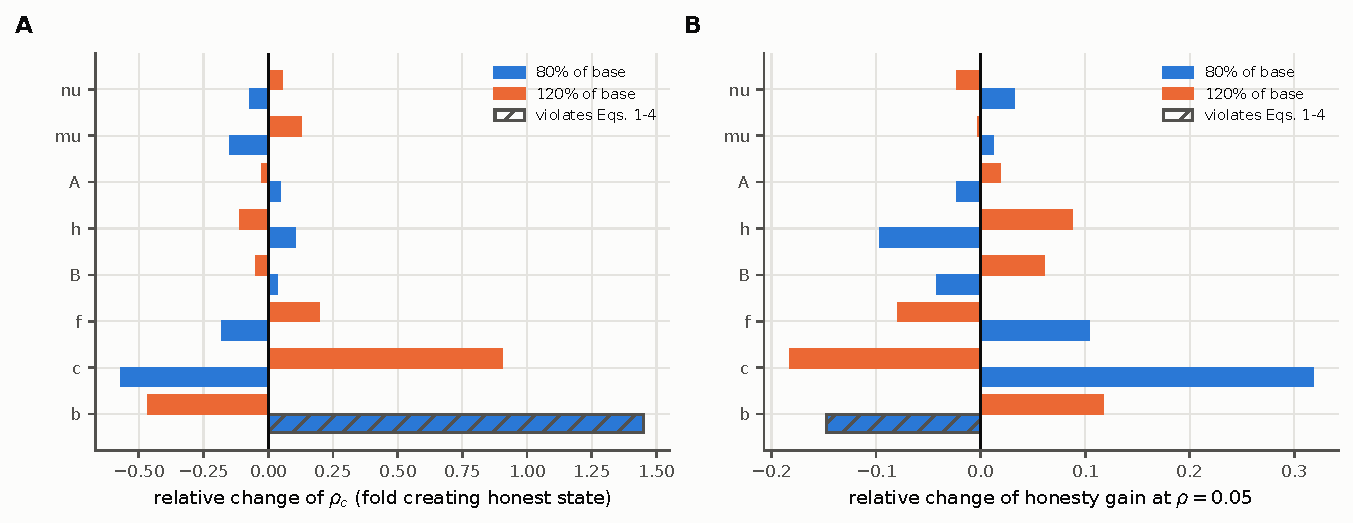
\includegraphics[width=0.85\textwidth]{figS2_sensitivity.pdf}
\caption{One-at-a-time sensitivity ($\pm20\%$) of (A) the critical rotation rate and (B) the gain
in honesty at $\rho=\RhoProbe$, mean field. Hatched bars violate the parameter conditions of Lee
et al.}
\label{fig:S2}
\end{figure*}

\begin{figure*}[!t]
\centering
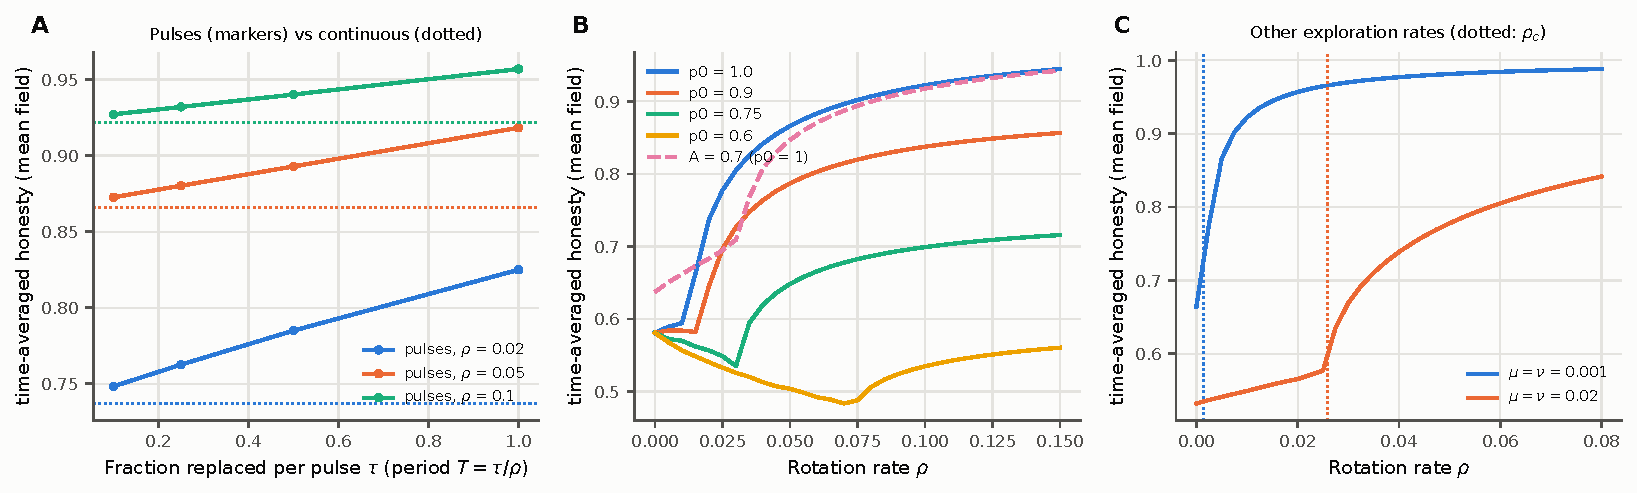
\includegraphics[width=\textwidth]{figS3_robustness.pdf}
\caption{Robustness. (A) Pulsed rotation (markers) against continuous rotation (dotted) at the
same average rate, mean field. (B) Newcomer honesty $p_0<1$ and $A=0.7$. (C) Exploration rates
$\mu=\nu=10^{-3}$ and $0.02$; dotted lines mark $\rhoc$.}
\label{fig:S3}
\end{figure*}

\section*{Data and Code Availability}
All code, configuration files, results (with configuration hashes and git commits), and the
scripts that generate every figure and number are available at [repository URL placeholder].

\section*{Acknowledgment}
[Placeholder.]

\bibliographystyle{IEEEtran}
\bibliography{refs_ieee}

\end{document}
